\documentclass[twoside]{book}

% Packages required by doxygen
\usepackage{fixltx2e}
\usepackage{calc}
\usepackage{doxygen}
\usepackage[export]{adjustbox} % also loads graphicx
\usepackage{graphicx}
\usepackage[utf8]{inputenc}
\usepackage{makeidx}
\usepackage{multicol}
\usepackage{multirow}
\PassOptionsToPackage{warn}{textcomp}
\usepackage{textcomp}
\usepackage[nointegrals]{wasysym}
\usepackage[table]{xcolor}

% Font selection
\usepackage[T1]{fontenc}
\usepackage[scaled=.90]{helvet}
\usepackage{courier}
\usepackage{amssymb}
\usepackage{sectsty}
\renewcommand{\familydefault}{\sfdefault}
\allsectionsfont{%
  \fontseries{bc}\selectfont%
  \color{darkgray}%
}
\renewcommand{\DoxyLabelFont}{%
  \fontseries{bc}\selectfont%
  \color{darkgray}%
}
\newcommand{\+}{\discretionary{\mbox{\scriptsize$\hookleftarrow$}}{}{}}

% Page & text layout
\usepackage{geometry}
\geometry{%
  a4paper,%
  top=2.5cm,%
  bottom=2.5cm,%
  left=2.5cm,%
  right=2.5cm%
}
\tolerance=750
\hfuzz=15pt
\hbadness=750
\setlength{\emergencystretch}{15pt}
\setlength{\parindent}{0cm}
\setlength{\parskip}{3ex plus 2ex minus 2ex}
\makeatletter
\renewcommand{\paragraph}{%
  \@startsection{paragraph}{4}{0ex}{-1.0ex}{1.0ex}{%
    \normalfont\normalsize\bfseries\SS@parafont%
  }%
}
\renewcommand{\subparagraph}{%
  \@startsection{subparagraph}{5}{0ex}{-1.0ex}{1.0ex}{%
    \normalfont\normalsize\bfseries\SS@subparafont%
  }%
}
\makeatother

% Headers & footers
\usepackage{fancyhdr}
\pagestyle{fancyplain}
\fancyhead[LE]{\fancyplain{}{\bfseries\thepage}}
\fancyhead[CE]{\fancyplain{}{}}
\fancyhead[RE]{\fancyplain{}{\bfseries\leftmark}}
\fancyhead[LO]{\fancyplain{}{\bfseries\rightmark}}
\fancyhead[CO]{\fancyplain{}{}}
\fancyhead[RO]{\fancyplain{}{\bfseries\thepage}}
\fancyfoot[LE]{\fancyplain{}{}}
\fancyfoot[CE]{\fancyplain{}{}}
\fancyfoot[RE]{\fancyplain{}{\bfseries\scriptsize Generated by Doxygen }}
\fancyfoot[LO]{\fancyplain{}{\bfseries\scriptsize Generated by Doxygen }}
\fancyfoot[CO]{\fancyplain{}{}}
\fancyfoot[RO]{\fancyplain{}{}}
\renewcommand{\footrulewidth}{0.4pt}
\renewcommand{\chaptermark}[1]{%
  \markboth{#1}{}%
}
\renewcommand{\sectionmark}[1]{%
  \markright{\thesection\ #1}%
}

% Indices & bibliography
\usepackage{natbib}
\usepackage[titles]{tocloft}
\setcounter{tocdepth}{3}
\setcounter{secnumdepth}{5}
\makeindex

% Hyperlinks (required, but should be loaded last)
\usepackage{ifpdf}
\ifpdf
  \usepackage[pdftex,pagebackref=true]{hyperref}
\else
  \usepackage[ps2pdf,pagebackref=true]{hyperref}
\fi
\hypersetup{%
  colorlinks=true,%
  linkcolor=blue,%
  citecolor=blue,%
  unicode%
}

% Custom commands
\newcommand{\clearemptydoublepage}{%
  \newpage{\pagestyle{empty}\cleardoublepage}%
}

\usepackage{caption}
\captionsetup{labelsep=space,justification=centering,font={bf},singlelinecheck=off,skip=4pt,position=top}

%===== C O N T E N T S =====

\begin{document}

% Titlepage & ToC
\hypersetup{pageanchor=false,
             bookmarksnumbered=true,
             pdfencoding=unicode
            }
\pagenumbering{roman}
\begin{titlepage}
\vspace*{7cm}
\begin{center}%
{\Large Polyomino \\[1ex]\large 0.\+1 }\\
\vspace*{1cm}
{\large Generated by Doxygen 1.8.11}\\
\end{center}
\end{titlepage}
\clearemptydoublepage
\tableofcontents
\clearemptydoublepage
\pagenumbering{arabic}
\hypersetup{pageanchor=true}

%--- Begin generated contents ---
\chapter{Hierarchical Index}
\section{Class Hierarchy}
This inheritance list is sorted roughly, but not completely, alphabetically\+:\begin{DoxyCompactList}
\item \contentsline{section}{matrix}{\pageref{classmatrix}}{}
\item Q\+Frame\begin{DoxyCompactList}
\item \contentsline{section}{Board}{\pageref{class_board}}{}
\item \contentsline{section}{Board2}{\pageref{class_board2}}{}
\end{DoxyCompactList}
\item Q\+Main\+Window\begin{DoxyCompactList}
\item \contentsline{section}{Main\+Window}{\pageref{class_main_window}}{}
\end{DoxyCompactList}
\item Q\+Widget\begin{DoxyCompactList}
\item \contentsline{section}{Window}{\pageref{class_window}}{}
\end{DoxyCompactList}
\item \contentsline{section}{Segment}{\pageref{class_segment}}{}
\item \contentsline{section}{Unit\+Cell}{\pageref{class_unit_cell}}{}
\end{DoxyCompactList}

\chapter{Class Index}
\section{Class List}
Here are the classes, structs, unions and interfaces with brief descriptions\+:\begin{DoxyCompactList}
\item\contentsline{section}{\hyperlink{class_board}{Board} \\*Classe representant le lecteur }{\pageref{class_board}}{}
\item\contentsline{section}{\hyperlink{class_board2}{Board2} \\*The \hyperlink{class_board2}{Board2} class dessine un polyomino à partir d\textquotesingle{}une liste de segments }{\pageref{class_board2}}{}
\item\contentsline{section}{\hyperlink{class_main_window}{Main\+Window} }{\pageref{class_main_window}}{}
\item\contentsline{section}{\hyperlink{classmatrix}{matrix} \\*The matrix class une matrice constituer de vecteur de vecteur }{\pageref{classmatrix}}{}
\item\contentsline{section}{\hyperlink{class_segment}{Segment} \\*The \hyperlink{class_segment}{Segment} class Représente un liste d\textquotesingle{}unicell }{\pageref{class_segment}}{}
\item\contentsline{section}{\hyperlink{class_unit_cell}{Unit\+Cell} \\*The \hyperlink{class_unit_cell}{Unit\+Cell} class contient la taille ,la couleur,et les coordonées d\textquotesingle{}une celluled\textquotesingle{}un polyomino }{\pageref{class_unit_cell}}{}
\item\contentsline{section}{\hyperlink{class_window}{Window} \\*The \hyperlink{class_window}{Window} class contient tous les widgets de l\textquotesingle{}application }{\pageref{class_window}}{}
\end{DoxyCompactList}

\chapter{File Index}
\section{File List}
Here is a list of all documented files with brief descriptions\+:\begin{DoxyCompactList}
\item\contentsline{section}{\hyperlink{board_8cpp}{board.\+cpp} \\*Gestion de la partie }{\pageref{board_8cpp}}{}
\item\contentsline{section}{\hyperlink{board_8h}{board.\+h} \\*Gestion de la partie }{\pageref{board_8h}}{}
\item\contentsline{section}{\hyperlink{board2_8cpp}{board2.\+cpp} \\*Représente le polyomino que l\textquotesingle{}on doit construire }{\pageref{board2_8cpp}}{}
\item\contentsline{section}{\hyperlink{board2_8h}{board2.\+h} \\*Représente le polyomino que l\textquotesingle{}on doit construire }{\pageref{board2_8h}}{}
\item\contentsline{section}{\hyperlink{main_8cpp}{main.\+cpp} \\*La main classe }{\pageref{main_8cpp}}{}
\item\contentsline{section}{{\bfseries mainwindow.\+h} }{\pageref{mainwindow_8h}}{}
\item\contentsline{section}{\hyperlink{matrix_8cpp}{matrix.\+cpp} \\*Gestion des déplacement }{\pageref{matrix_8cpp}}{}
\item\contentsline{section}{\hyperlink{matrix_8h}{matrix.\+h} \\*Gestion des déplacement }{\pageref{matrix_8h}}{}
\item\contentsline{section}{\hyperlink{segment_8cpp}{segment.\+cpp} \\*Représente une partie du polyomino }{\pageref{segment_8cpp}}{}
\item\contentsline{section}{\hyperlink{segment_8h}{segment.\+h} \\*Représente une partie du polyomino }{\pageref{segment_8h}}{}
\item\contentsline{section}{\hyperlink{unitcell_8cpp}{unitcell.\+cpp} \\*Représente une cellule de polyomino }{\pageref{unitcell_8cpp}}{}
\item\contentsline{section}{\hyperlink{unitcell_8h}{unitcell.\+h} \\*Représente une cellule de polyomino }{\pageref{unitcell_8h}}{}
\item\contentsline{section}{\hyperlink{window_8cpp}{window.\+cpp} \\*Représente l\textquotesingle{}interface graphique de l\textquotesingle{}application }{\pageref{window_8cpp}}{}
\item\contentsline{section}{\hyperlink{window_8h}{window.\+h} \\*Représente l\textquotesingle{}interface graphique de l\textquotesingle{}application }{\pageref{window_8h}}{}
\end{DoxyCompactList}

\chapter{Class Documentation}
\hypertarget{class_board}{}\section{Board Class Reference}
\label{class_board}\index{Board@{Board}}


classe representant le lecteur  




{\ttfamily \#include $<$board.\+h$>$}

Inheritance diagram for Board\+:\begin{figure}[H]
\begin{center}
\leavevmode
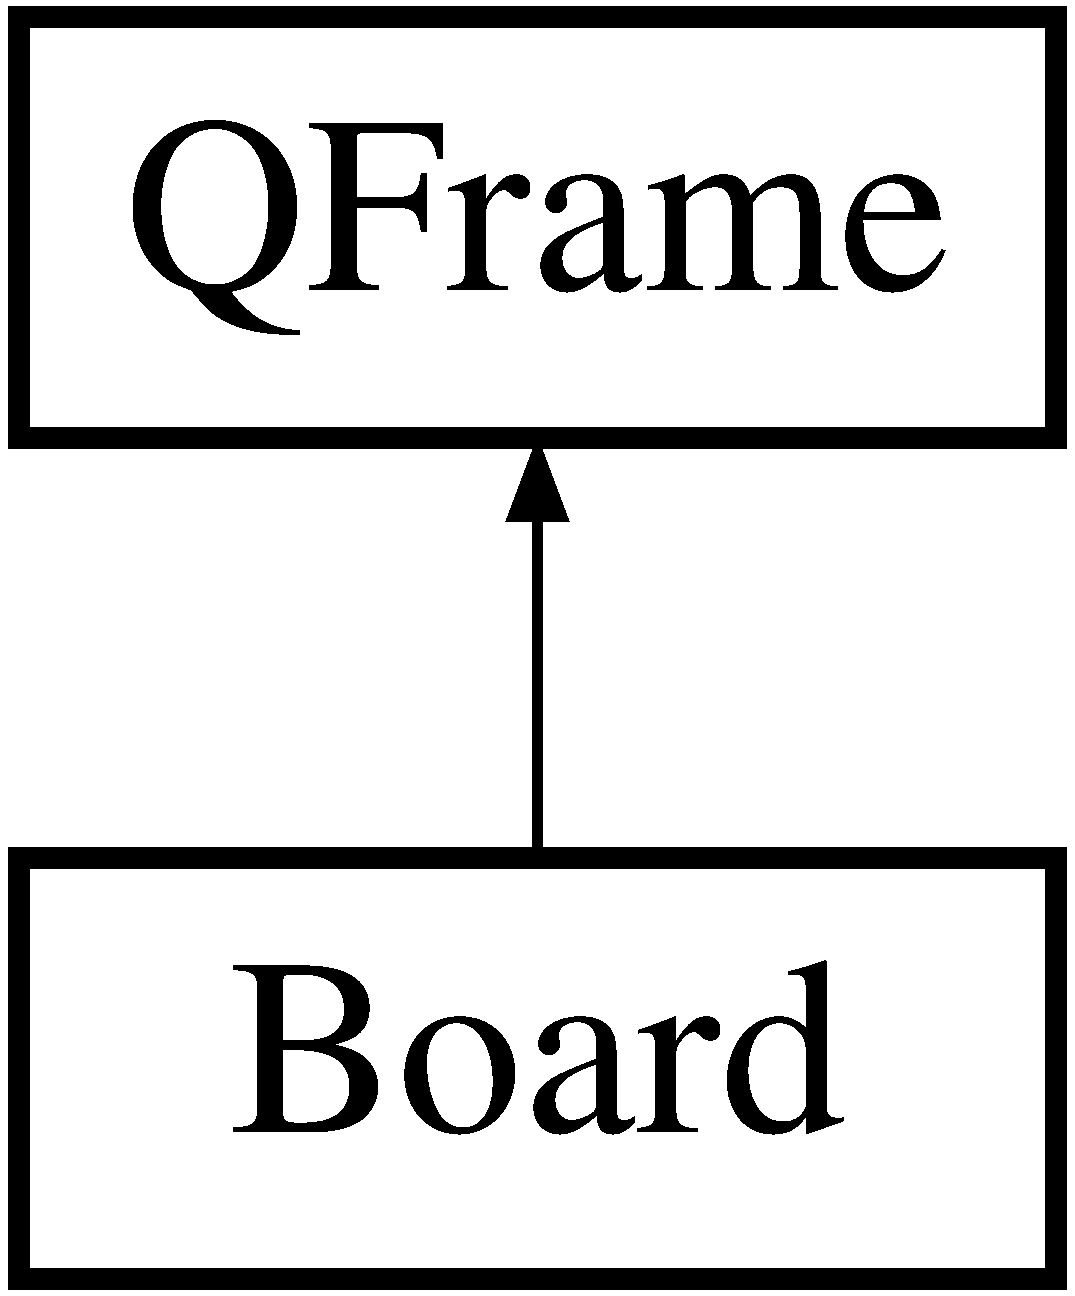
\includegraphics[height=2.000000cm]{class_board}
\end{center}
\end{figure}
\subsection*{Public Slots}
\begin{DoxyCompactItemize}
\item 
void \hyperlink{class_board_abb3ae1723d9e7a7a21cda3eb785b984a}{start} ()\hypertarget{class_board_abb3ae1723d9e7a7a21cda3eb785b984a}{}\label{class_board_abb3ae1723d9e7a7a21cda3eb785b984a}

\begin{DoxyCompactList}\small\item\em start lance la partie \end{DoxyCompactList}\item 
void \hyperlink{class_board_a4fa366b8eaa9151e1f16d37da8100f45}{pause} ()\hypertarget{class_board_a4fa366b8eaa9151e1f16d37da8100f45}{}\label{class_board_a4fa366b8eaa9151e1f16d37da8100f45}

\begin{DoxyCompactList}\small\item\em pause met en pause la partie \end{DoxyCompactList}\end{DoxyCompactItemize}
\subsection*{Signals}
\begin{DoxyCompactItemize}
\item 
void \hyperlink{class_board_a53590f45499231a01a8abbc9a95e396d}{score\+Changed} (int \hyperlink{class_board_a7a44f4be355783a0136e42c79733724a}{score})
\begin{DoxyCompactList}\small\item\em score\+Changed envoie le score au widget d\textquotesingle{}affichage du score \end{DoxyCompactList}\end{DoxyCompactItemize}
\subsection*{Public Member Functions}
\begin{DoxyCompactItemize}
\item 
void \hyperlink{class_board_a69e3222342a38b98d4d82522921164ba}{key\+Press\+Event} (Q\+Key\+Event $\ast$event)
\begin{DoxyCompactList}\small\item\em key\+Press\+Event gére le mouvement avec les touches du clavier \end{DoxyCompactList}\item 
int \hyperlink{class_board_af032dd7048b8e3532ffa65889919f23a}{square\+Width} ()
\begin{DoxyCompactList}\small\item\em square\+Width definit la taille d\textquotesingle{}une case d\textquotesingle{}un polyominos \end{DoxyCompactList}\item 
int \hyperlink{class_board_a1a4c3c20cfc820ce5b79d7ab01257890}{square\+Height} ()
\begin{DoxyCompactList}\small\item\em square\+Height definit la taille d\textquotesingle{}une case d\textquotesingle{}un polyominos \end{DoxyCompactList}\item 
\hyperlink{class_board_ace54d4a0f5ccec30c4c86e676299ccbf}{Board} (Q\+Widget $\ast$parent=0)
\begin{DoxyCompactList}\small\item\em \hyperlink{class_board}{Board} constructeur. \end{DoxyCompactList}\item 
void \hyperlink{class_board_a1a44a8a95cb3d04207db592f913db009}{timer\+Event} (Q\+Timer\+Event $\ast$event)
\begin{DoxyCompactList}\small\item\em timer\+Event appelle les fonctions motrices du jeu toutes les 1 secondes \end{DoxyCompactList}\item 
bool \hyperlink{class_board_a4fd044f03afc199a0825635d8485f93f}{try\+MoveR} (\hyperlink{class_segment}{Segment} $\ast$segment)
\begin{DoxyCompactList}\small\item\em try\+MoveR verifie qu\textquotesingle{}un segment à le doit de se déplacer vert la droite \end{DoxyCompactList}\item 
bool \hyperlink{class_board_a58ab26b2c4e2dbc3312a95261b282adf}{try\+MoveL} (\hyperlink{class_segment}{Segment} $\ast$segment)
\begin{DoxyCompactList}\small\item\em try\+MoveL verifie qu\textquotesingle{}un segment à le doit de se déplacer vert la gauche \end{DoxyCompactList}\item 
Q\+Size {\bfseries size\+Hint} () const Q\+\_\+\+D\+E\+C\+L\+\_\+\+O\+V\+E\+R\+R\+I\+DE\hypertarget{class_board_a3a8c20b7452b2faf9cb9b9062c608113}{}\label{class_board_a3a8c20b7452b2faf9cb9b9062c608113}

\item 
Q\+Size {\bfseries minimum\+Size\+Hint} () const Q\+\_\+\+D\+E\+C\+L\+\_\+\+O\+V\+E\+R\+R\+I\+DE\hypertarget{class_board_a7073de6d1a8c9feeca5ed7d14361c113}{}\label{class_board_a7073de6d1a8c9feeca5ed7d14361c113}

\item 
void \hyperlink{class_board_af518da96919d04d1f0dbe0794b61d532}{paint\+Event} (Q\+Paint\+Event $\ast$event)
\begin{DoxyCompactList}\small\item\em paint\+Event permet de dessiner les polyominos \end{DoxyCompactList}\item 
bool \hyperlink{class_board_af4ac464e41d36aeaa587cb03ce6fec34}{try\+Move} (\hyperlink{class_segment}{Segment} $\ast$segment)
\begin{DoxyCompactList}\small\item\em try\+Move verifie qu\textquotesingle{}un segment à le doit de se déplacer vers le bas \end{DoxyCompactList}\item 
void \hyperlink{class_board_a1211e4f86b63cdeacb2f7aed16ca650f}{move} (int movement)
\begin{DoxyCompactList}\small\item\em move effectie le mouvement \end{DoxyCompactList}\item 
void \hyperlink{class_board_a7c04c8ddb76471bff762229c079c9614}{col\+Gen} (bool f)
\begin{DoxyCompactList}\small\item\em col\+Gen génère un polyomino en forme de barre de taille aléatoire \end{DoxyCompactList}\item 
bool \hyperlink{class_board_a65c546b6f6c5904306174afcbe55a2bb}{is\+Paused} () const 
\begin{DoxyCompactList}\small\item\em is\+Paused renvoie true si le jeu est en pause \end{DoxyCompactList}\item 
bool \hyperlink{class_board_ad811426191e931d672c056339935b602}{is\+Started} () const 
\begin{DoxyCompactList}\small\item\em is\+Started renvoie true si le jeu à commencer \end{DoxyCompactList}\item 
bool \hyperlink{class_board_a8759b41634150be8a0b7767f59d93acd}{polyo} ()
\begin{DoxyCompactList}\small\item\em polyo verifie si c\textquotesingle{}est un polyomino \end{DoxyCompactList}\item 
void \hyperlink{class_board_a9e49166a714ab1f7f5f7ab5035e05784}{update\+Board} (\hyperlink{class_segment}{Segment} $\ast$segment)
\begin{DoxyCompactList}\small\item\em update\+Board met a jour le board et affichage d\textquotesingle{}informations \end{DoxyCompactList}\item 
bool \hyperlink{class_board_a1884990eae00d36ff465bed7df8ce4fe}{prefix\+Closed} ()
\begin{DoxyCompactList}\small\item\em prefix\+Closed verifie si le poyomino est bien prefixe close \end{DoxyCompactList}\item 
bool \hyperlink{class_board_aea9fad5f32155cf8c6b16254e072f6bd}{try\+Rotate} (\hyperlink{class_segment}{Segment} $\ast$segment)
\begin{DoxyCompactList}\small\item\em try\+Rotate verifie que le segment peut faire une rorarion \end{DoxyCompactList}\item 
void \hyperlink{class_board_af74f0d4b43e5aa3faea16d7c6407b05e}{clear} ()\hypertarget{class_board_af74f0d4b43e5aa3faea16d7c6407b05e}{}\label{class_board_af74f0d4b43e5aa3faea16d7c6407b05e}

\begin{DoxyCompactList}\small\item\em clear nettoie le board \end{DoxyCompactList}\end{DoxyCompactItemize}
\subsection*{Public Attributes}
\begin{DoxyCompactItemize}
\item 
int \hyperlink{class_board_a81859b3ab8f00f4c74fd89d0db0ca412}{board\+Height} =25\hypertarget{class_board_a81859b3ab8f00f4c74fd89d0db0ca412}{}\label{class_board_a81859b3ab8f00f4c74fd89d0db0ca412}

\begin{DoxyCompactList}\small\item\em board\+Height taille en hauteur du board \end{DoxyCompactList}\item 
int \hyperlink{class_board_a3aa771a6eb106b66525123a3d72ab1b7}{board\+Width} =25\hypertarget{class_board_a3aa771a6eb106b66525123a3d72ab1b7}{}\label{class_board_a3aa771a6eb106b66525123a3d72ab1b7}

\begin{DoxyCompactList}\small\item\em board\+Width taille en largeur du board \end{DoxyCompactList}\item 
int \hyperlink{class_board_a7a44f4be355783a0136e42c79733724a}{score} =0\hypertarget{class_board_a7a44f4be355783a0136e42c79733724a}{}\label{class_board_a7a44f4be355783a0136e42c79733724a}

\begin{DoxyCompactList}\small\item\em score score de la partie \end{DoxyCompactList}\item 
bool \hyperlink{class_board_afdb871d4bd6f37e1a98564745d762420}{fini} =false\hypertarget{class_board_afdb871d4bd6f37e1a98564745d762420}{}\label{class_board_afdb871d4bd6f37e1a98564745d762420}

\begin{DoxyCompactList}\small\item\em fini definit si une parite est fini \end{DoxyCompactList}\item 
int \hyperlink{class_board_a424cefa1387e098268b6be64e738ca31}{acc} =0
\begin{DoxyCompactList}\small\item\em timer timer du widget \end{DoxyCompactList}\item 
Q\+Basic\+Timer {\bfseries timer}\hypertarget{class_board_a2ff086910f4575f5fdfb1378c56f262f}{}\label{class_board_a2ff086910f4575f5fdfb1378c56f262f}

\item 
\hyperlink{classmatrix}{matrix} $\ast$ \hyperlink{class_board_aaba5e7fbe2ca37b151abcf08fe5a48cd}{board}\hypertarget{class_board_aaba5e7fbe2ca37b151abcf08fe5a48cd}{}\label{class_board_aaba5e7fbe2ca37b151abcf08fe5a48cd}

\begin{DoxyCompactList}\small\item\em board représente les polyominos sous forme d\textquotesingle{}une matrice de 0 et de 1 \end{DoxyCompactList}\item 
\hyperlink{class_segment}{Segment} $\ast$ \hyperlink{class_board_a3f7976a204967a943d0c5a464ddad6a3}{cur\+Segment} = N\+U\+LL\hypertarget{class_board_a3f7976a204967a943d0c5a464ddad6a3}{}\label{class_board_a3f7976a204967a943d0c5a464ddad6a3}

\begin{DoxyCompactList}\small\item\em cur\+Segment le segment qui est entrain d\textquotesingle{}être poser \end{DoxyCompactList}\item 
std\+::vector$<$ \hyperlink{class_segment}{Segment} $>$ \hyperlink{class_board_ace42dd2bb49a49cfa537b218e03b52fd}{segments}\hypertarget{class_board_ace42dd2bb49a49cfa537b218e03b52fd}{}\label{class_board_ace42dd2bb49a49cfa537b218e03b52fd}

\begin{DoxyCompactList}\small\item\em segments liste des segments deja posé \end{DoxyCompactList}\item 
bool \hyperlink{class_board_aeadc14404bfb8ce40d0ca3736c7db5f6}{paused} = false\hypertarget{class_board_aeadc14404bfb8ce40d0ca3736c7db5f6}{}\label{class_board_aeadc14404bfb8ce40d0ca3736c7db5f6}

\begin{DoxyCompactList}\small\item\em paused definit si la partie est en pause \end{DoxyCompactList}\item 
bool \hyperlink{class_board_a357bd6048217a80d0773c404ddc1dee9}{started} = false\hypertarget{class_board_a357bd6048217a80d0773c404ddc1dee9}{}\label{class_board_a357bd6048217a80d0773c404ddc1dee9}

\begin{DoxyCompactList}\small\item\em started definit si la partie est lancé \end{DoxyCompactList}\item 
bool \hyperlink{class_board_a4accd5b6bccf3ce151e6ffc12fa26552}{segment\+Dropped} = false\hypertarget{class_board_a4accd5b6bccf3ce151e6ffc12fa26552}{}\label{class_board_a4accd5b6bccf3ce151e6ffc12fa26552}

\begin{DoxyCompactList}\small\item\em segment\+Dropped definit si le segment courant a été posé \end{DoxyCompactList}\end{DoxyCompactItemize}


\subsection{Detailed Description}
classe representant le lecteur 

La classe gere l\textquotesingle{}affichage et le deroulement de la partie 

\subsection{Constructor \& Destructor Documentation}
\index{Board@{Board}!Board@{Board}}
\index{Board@{Board}!Board@{Board}}
\subsubsection[{\texorpdfstring{Board(\+Q\+Widget $\ast$parent=0)}{Board(QWidget *parent=0)}}]{\setlength{\rightskip}{0pt plus 5cm}Board\+::\+Board (
\begin{DoxyParamCaption}
\item[{Q\+Widget $\ast$}]{parent = {\ttfamily 0}}
\end{DoxyParamCaption}
)}\hypertarget{class_board_ace54d4a0f5ccec30c4c86e676299ccbf}{}\label{class_board_ace54d4a0f5ccec30c4c86e676299ccbf}


\hyperlink{class_board}{Board} constructeur. 


\begin{DoxyParams}{Parameters}
{\em parent} & \\
\hline
\end{DoxyParams}


\subsection{Member Function Documentation}
\index{Board@{Board}!col\+Gen@{col\+Gen}}
\index{col\+Gen@{col\+Gen}!Board@{Board}}
\subsubsection[{\texorpdfstring{col\+Gen(bool f)}{colGen(bool f)}}]{\setlength{\rightskip}{0pt plus 5cm}void Board\+::col\+Gen (
\begin{DoxyParamCaption}
\item[{bool}]{f}
\end{DoxyParamCaption}
)}\hypertarget{class_board_a7c04c8ddb76471bff762229c079c9614}{}\label{class_board_a7c04c8ddb76471bff762229c079c9614}


col\+Gen génère un polyomino en forme de barre de taille aléatoire 


\begin{DoxyParams}{Parameters}
{\em f} & sa position verticale ou horizontale \\
\hline
\end{DoxyParams}
\index{Board@{Board}!is\+Paused@{is\+Paused}}
\index{is\+Paused@{is\+Paused}!Board@{Board}}
\subsubsection[{\texorpdfstring{is\+Paused() const }{isPaused() const }}]{\setlength{\rightskip}{0pt plus 5cm}bool Board\+::is\+Paused (
\begin{DoxyParamCaption}
{}
\end{DoxyParamCaption}
) const\hspace{0.3cm}{\ttfamily [inline]}}\hypertarget{class_board_a65c546b6f6c5904306174afcbe55a2bb}{}\label{class_board_a65c546b6f6c5904306174afcbe55a2bb}


is\+Paused renvoie true si le jeu est en pause 

\begin{DoxyReturn}{Returns}

\end{DoxyReturn}
\index{Board@{Board}!is\+Started@{is\+Started}}
\index{is\+Started@{is\+Started}!Board@{Board}}
\subsubsection[{\texorpdfstring{is\+Started() const }{isStarted() const }}]{\setlength{\rightskip}{0pt plus 5cm}bool Board\+::is\+Started (
\begin{DoxyParamCaption}
{}
\end{DoxyParamCaption}
) const\hspace{0.3cm}{\ttfamily [inline]}}\hypertarget{class_board_ad811426191e931d672c056339935b602}{}\label{class_board_ad811426191e931d672c056339935b602}


is\+Started renvoie true si le jeu à commencer 

\begin{DoxyReturn}{Returns}

\end{DoxyReturn}
\index{Board@{Board}!key\+Press\+Event@{key\+Press\+Event}}
\index{key\+Press\+Event@{key\+Press\+Event}!Board@{Board}}
\subsubsection[{\texorpdfstring{key\+Press\+Event(\+Q\+Key\+Event $\ast$event)}{keyPressEvent(QKeyEvent *event)}}]{\setlength{\rightskip}{0pt plus 5cm}void Board\+::key\+Press\+Event (
\begin{DoxyParamCaption}
\item[{Q\+Key\+Event $\ast$}]{event}
\end{DoxyParamCaption}
)}\hypertarget{class_board_a69e3222342a38b98d4d82522921164ba}{}\label{class_board_a69e3222342a38b98d4d82522921164ba}


key\+Press\+Event gére le mouvement avec les touches du clavier 


\begin{DoxyParams}{Parameters}
{\em event} & \\
\hline
\end{DoxyParams}
\index{Board@{Board}!move@{move}}
\index{move@{move}!Board@{Board}}
\subsubsection[{\texorpdfstring{move(int movement)}{move(int movement)}}]{\setlength{\rightskip}{0pt plus 5cm}void Board\+::move (
\begin{DoxyParamCaption}
\item[{int}]{movement}
\end{DoxyParamCaption}
)}\hypertarget{class_board_a1211e4f86b63cdeacb2f7aed16ca650f}{}\label{class_board_a1211e4f86b63cdeacb2f7aed16ca650f}


move effectie le mouvement 


\begin{DoxyParams}{Parameters}
{\em movement} & \\
\hline
\end{DoxyParams}
\index{Board@{Board}!paint\+Event@{paint\+Event}}
\index{paint\+Event@{paint\+Event}!Board@{Board}}
\subsubsection[{\texorpdfstring{paint\+Event(\+Q\+Paint\+Event $\ast$event)}{paintEvent(QPaintEvent *event)}}]{\setlength{\rightskip}{0pt plus 5cm}void Board\+::paint\+Event (
\begin{DoxyParamCaption}
\item[{Q\+Paint\+Event $\ast$}]{event}
\end{DoxyParamCaption}
)}\hypertarget{class_board_af518da96919d04d1f0dbe0794b61d532}{}\label{class_board_af518da96919d04d1f0dbe0794b61d532}


paint\+Event permet de dessiner les polyominos 


\begin{DoxyParams}{Parameters}
{\em event} & \\
\hline
\end{DoxyParams}
\index{Board@{Board}!polyo@{polyo}}
\index{polyo@{polyo}!Board@{Board}}
\subsubsection[{\texorpdfstring{polyo()}{polyo()}}]{\setlength{\rightskip}{0pt plus 5cm}bool Board\+::polyo (
\begin{DoxyParamCaption}
{}
\end{DoxyParamCaption}
)}\hypertarget{class_board_a8759b41634150be8a0b7767f59d93acd}{}\label{class_board_a8759b41634150be8a0b7767f59d93acd}


polyo verifie si c\textquotesingle{}est un polyomino 

\begin{DoxyReturn}{Returns}

\end{DoxyReturn}
\index{Board@{Board}!prefix\+Closed@{prefix\+Closed}}
\index{prefix\+Closed@{prefix\+Closed}!Board@{Board}}
\subsubsection[{\texorpdfstring{prefix\+Closed()}{prefixClosed()}}]{\setlength{\rightskip}{0pt plus 5cm}bool Board\+::prefix\+Closed (
\begin{DoxyParamCaption}
{}
\end{DoxyParamCaption}
)}\hypertarget{class_board_a1884990eae00d36ff465bed7df8ce4fe}{}\label{class_board_a1884990eae00d36ff465bed7df8ce4fe}


prefix\+Closed verifie si le poyomino est bien prefixe close 

\begin{DoxyReturn}{Returns}

\end{DoxyReturn}
\index{Board@{Board}!score\+Changed@{score\+Changed}}
\index{score\+Changed@{score\+Changed}!Board@{Board}}
\subsubsection[{\texorpdfstring{score\+Changed}{scoreChanged}}]{\setlength{\rightskip}{0pt plus 5cm}void Board\+::score\+Changed (
\begin{DoxyParamCaption}
\item[{int}]{score}
\end{DoxyParamCaption}
)\hspace{0.3cm}{\ttfamily [signal]}}\hypertarget{class_board_a53590f45499231a01a8abbc9a95e396d}{}\label{class_board_a53590f45499231a01a8abbc9a95e396d}


score\+Changed envoie le score au widget d\textquotesingle{}affichage du score 


\begin{DoxyParams}{Parameters}
{\em score} & \\
\hline
\end{DoxyParams}
\index{Board@{Board}!square\+Height@{square\+Height}}
\index{square\+Height@{square\+Height}!Board@{Board}}
\subsubsection[{\texorpdfstring{square\+Height()}{squareHeight()}}]{\setlength{\rightskip}{0pt plus 5cm}int Board\+::square\+Height (
\begin{DoxyParamCaption}
{}
\end{DoxyParamCaption}
)\hspace{0.3cm}{\ttfamily [inline]}}\hypertarget{class_board_a1a4c3c20cfc820ce5b79d7ab01257890}{}\label{class_board_a1a4c3c20cfc820ce5b79d7ab01257890}


square\+Height definit la taille d\textquotesingle{}une case d\textquotesingle{}un polyominos 

\begin{DoxyReturn}{Returns}

\end{DoxyReturn}
\index{Board@{Board}!square\+Width@{square\+Width}}
\index{square\+Width@{square\+Width}!Board@{Board}}
\subsubsection[{\texorpdfstring{square\+Width()}{squareWidth()}}]{\setlength{\rightskip}{0pt plus 5cm}int Board\+::square\+Width (
\begin{DoxyParamCaption}
{}
\end{DoxyParamCaption}
)\hspace{0.3cm}{\ttfamily [inline]}}\hypertarget{class_board_af032dd7048b8e3532ffa65889919f23a}{}\label{class_board_af032dd7048b8e3532ffa65889919f23a}


square\+Width definit la taille d\textquotesingle{}une case d\textquotesingle{}un polyominos 

\begin{DoxyReturn}{Returns}

\end{DoxyReturn}
\index{Board@{Board}!timer\+Event@{timer\+Event}}
\index{timer\+Event@{timer\+Event}!Board@{Board}}
\subsubsection[{\texorpdfstring{timer\+Event(\+Q\+Timer\+Event $\ast$event)}{timerEvent(QTimerEvent *event)}}]{\setlength{\rightskip}{0pt plus 5cm}void Board\+::timer\+Event (
\begin{DoxyParamCaption}
\item[{Q\+Timer\+Event $\ast$}]{event}
\end{DoxyParamCaption}
)}\hypertarget{class_board_a1a44a8a95cb3d04207db592f913db009}{}\label{class_board_a1a44a8a95cb3d04207db592f913db009}


timer\+Event appelle les fonctions motrices du jeu toutes les 1 secondes 


\begin{DoxyParams}{Parameters}
{\em event} & \\
\hline
\end{DoxyParams}
\index{Board@{Board}!try\+Move@{try\+Move}}
\index{try\+Move@{try\+Move}!Board@{Board}}
\subsubsection[{\texorpdfstring{try\+Move(\+Segment $\ast$segment)}{tryMove(Segment *segment)}}]{\setlength{\rightskip}{0pt plus 5cm}bool Board\+::try\+Move (
\begin{DoxyParamCaption}
\item[{{\bf Segment} $\ast$}]{segment}
\end{DoxyParamCaption}
)}\hypertarget{class_board_af4ac464e41d36aeaa587cb03ce6fec34}{}\label{class_board_af4ac464e41d36aeaa587cb03ce6fec34}


try\+Move verifie qu\textquotesingle{}un segment à le doit de se déplacer vers le bas 


\begin{DoxyParams}{Parameters}
{\em segment} & \\
\hline
\end{DoxyParams}
\begin{DoxyReturn}{Returns}

\end{DoxyReturn}
\index{Board@{Board}!try\+MoveL@{try\+MoveL}}
\index{try\+MoveL@{try\+MoveL}!Board@{Board}}
\subsubsection[{\texorpdfstring{try\+Move\+L(\+Segment $\ast$segment)}{tryMoveL(Segment *segment)}}]{\setlength{\rightskip}{0pt plus 5cm}bool Board\+::try\+MoveL (
\begin{DoxyParamCaption}
\item[{{\bf Segment} $\ast$}]{segment}
\end{DoxyParamCaption}
)}\hypertarget{class_board_a58ab26b2c4e2dbc3312a95261b282adf}{}\label{class_board_a58ab26b2c4e2dbc3312a95261b282adf}


try\+MoveL verifie qu\textquotesingle{}un segment à le doit de se déplacer vert la gauche 


\begin{DoxyParams}{Parameters}
{\em segment} & \\
\hline
\end{DoxyParams}
\begin{DoxyReturn}{Returns}

\end{DoxyReturn}
\index{Board@{Board}!try\+MoveR@{try\+MoveR}}
\index{try\+MoveR@{try\+MoveR}!Board@{Board}}
\subsubsection[{\texorpdfstring{try\+Move\+R(\+Segment $\ast$segment)}{tryMoveR(Segment *segment)}}]{\setlength{\rightskip}{0pt plus 5cm}bool Board\+::try\+MoveR (
\begin{DoxyParamCaption}
\item[{{\bf Segment} $\ast$}]{segment}
\end{DoxyParamCaption}
)}\hypertarget{class_board_a4fd044f03afc199a0825635d8485f93f}{}\label{class_board_a4fd044f03afc199a0825635d8485f93f}


try\+MoveR verifie qu\textquotesingle{}un segment à le doit de se déplacer vert la droite 


\begin{DoxyParams}{Parameters}
{\em segment} & \\
\hline
\end{DoxyParams}
\begin{DoxyReturn}{Returns}

\end{DoxyReturn}
\index{Board@{Board}!try\+Rotate@{try\+Rotate}}
\index{try\+Rotate@{try\+Rotate}!Board@{Board}}
\subsubsection[{\texorpdfstring{try\+Rotate(\+Segment $\ast$segment)}{tryRotate(Segment *segment)}}]{\setlength{\rightskip}{0pt plus 5cm}bool Board\+::try\+Rotate (
\begin{DoxyParamCaption}
\item[{{\bf Segment} $\ast$}]{segment}
\end{DoxyParamCaption}
)}\hypertarget{class_board_aea9fad5f32155cf8c6b16254e072f6bd}{}\label{class_board_aea9fad5f32155cf8c6b16254e072f6bd}


try\+Rotate verifie que le segment peut faire une rorarion 


\begin{DoxyParams}{Parameters}
{\em segment} & \\
\hline
\end{DoxyParams}
\begin{DoxyReturn}{Returns}

\end{DoxyReturn}
\index{Board@{Board}!update\+Board@{update\+Board}}
\index{update\+Board@{update\+Board}!Board@{Board}}
\subsubsection[{\texorpdfstring{update\+Board(\+Segment $\ast$segment)}{updateBoard(Segment *segment)}}]{\setlength{\rightskip}{0pt plus 5cm}void Board\+::update\+Board (
\begin{DoxyParamCaption}
\item[{{\bf Segment} $\ast$}]{segment}
\end{DoxyParamCaption}
)}\hypertarget{class_board_a9e49166a714ab1f7f5f7ab5035e05784}{}\label{class_board_a9e49166a714ab1f7f5f7ab5035e05784}


update\+Board met a jour le board et affichage d\textquotesingle{}informations 


\begin{DoxyParams}{Parameters}
{\em segment} & \\
\hline
\end{DoxyParams}


\subsection{Member Data Documentation}
\index{Board@{Board}!acc@{acc}}
\index{acc@{acc}!Board@{Board}}
\subsubsection[{\texorpdfstring{acc}{acc}}]{\setlength{\rightskip}{0pt plus 5cm}int Board\+::acc =0}\hypertarget{class_board_a424cefa1387e098268b6be64e738ca31}{}\label{class_board_a424cefa1387e098268b6be64e738ca31}


timer timer du widget 

acc compte le nombre de piece posé 

The documentation for this class was generated from the following files\+:\begin{DoxyCompactItemize}
\item 
\hyperlink{board_8h}{board.\+h}\item 
\hyperlink{board_8cpp}{board.\+cpp}\end{DoxyCompactItemize}

\hypertarget{class_board2}{}\section{Board2 Class Reference}
\label{class_board2}\index{Board2@{Board2}}


The \hyperlink{class_board2}{Board2} class dessine un polyomino à partir d\textquotesingle{}une liste de segments.  




{\ttfamily \#include $<$board2.\+h$>$}

Inheritance diagram for Board2\+:\begin{figure}[H]
\begin{center}
\leavevmode
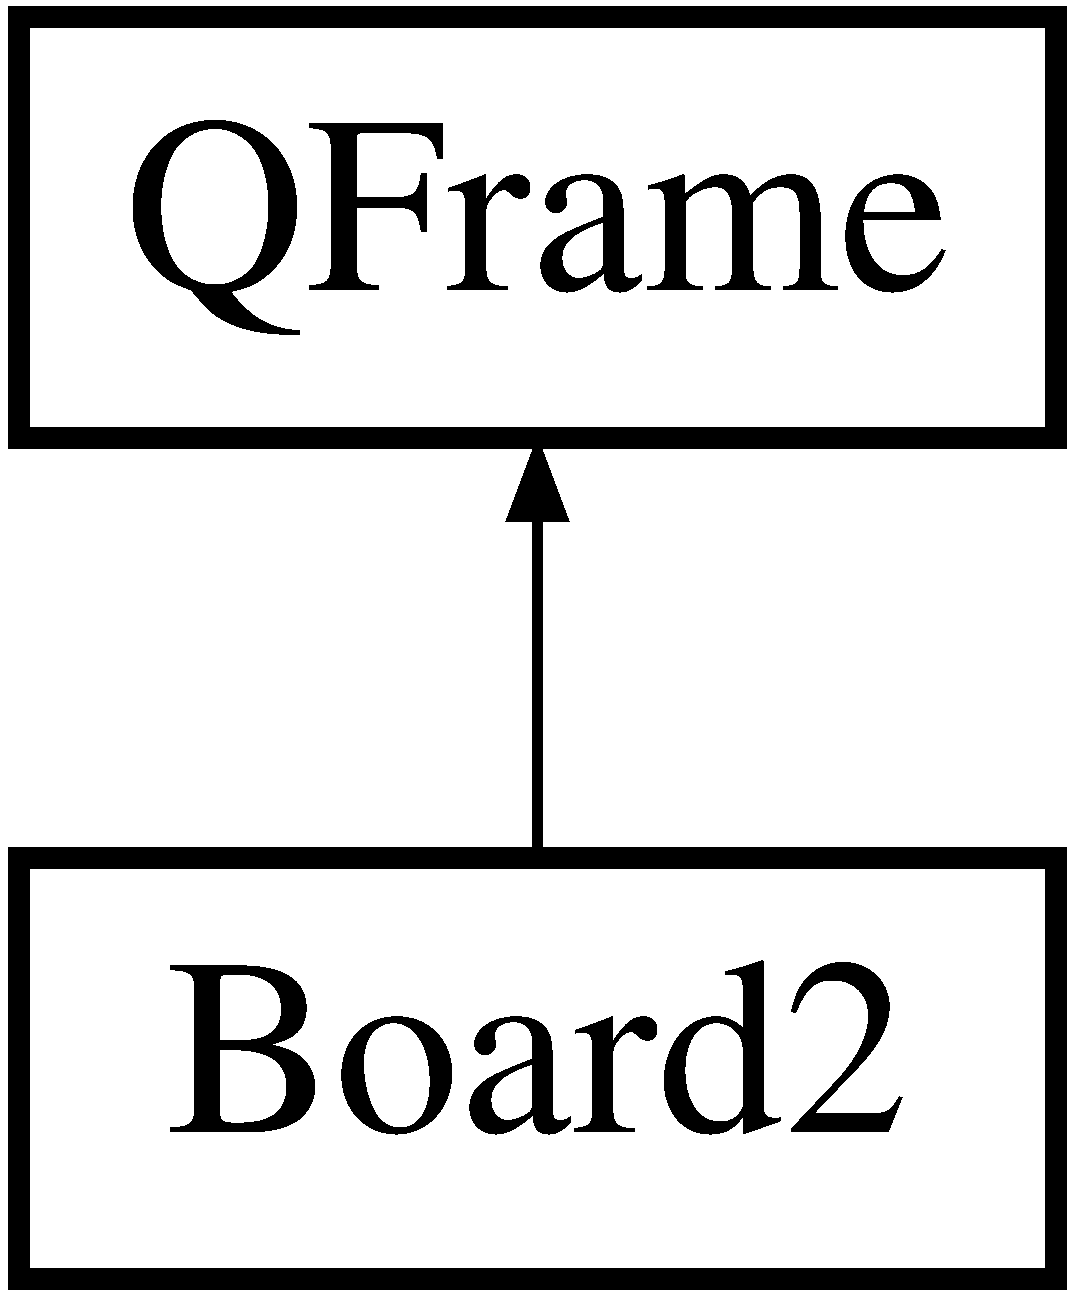
\includegraphics[height=2.000000cm]{class_board2}
\end{center}
\end{figure}
\subsection*{Public Slots}
\begin{DoxyCompactItemize}
\item 
void {\bfseries start} ()\hypertarget{class_board2_ab7dff7e5274b356a9e6fcf86504d83ff}{}\label{class_board2_ab7dff7e5274b356a9e6fcf86504d83ff}

\end{DoxyCompactItemize}
\subsection*{Public Member Functions}
\begin{DoxyCompactItemize}
\item 
\hyperlink{class_board2_aae64d4a675128c16c00d07149c1a4ee3}{Board2} (Q\+Widget $\ast$parent=0)
\begin{DoxyCompactList}\small\item\em \hyperlink{class_board2}{Board2} constructeur. \end{DoxyCompactList}\item 
int {\bfseries square\+Width} ()\hypertarget{class_board2_a427244655bbee1815563d39858dc0fa3}{}\label{class_board2_a427244655bbee1815563d39858dc0fa3}

\item 
int {\bfseries square\+Height} ()\hypertarget{class_board2_a7c2b21739e7afcd6442b1d9e4c822ad5}{}\label{class_board2_a7c2b21739e7afcd6442b1d9e4c822ad5}

\item 
void \hyperlink{class_board2_af4b54598413c7146ae1281ffb0da1002}{timer\+Event} (Q\+Timer\+Event $\ast$event)
\begin{DoxyCompactList}\small\item\em timer\+Event achange de polyomino toutes les 1 secondes \end{DoxyCompactList}\item 
void \hyperlink{class_board2_a5457e120d690a6706c1e9f2949777721}{paint\+Event} (Q\+Paint\+Event $\ast$event)
\begin{DoxyCompactList}\small\item\em paint\+Event dessine le polyiomino \end{DoxyCompactList}\item 
void \hyperlink{class_board2_ab02675377010f5f137a5d34f013ffc42}{lecture} ()\hypertarget{class_board2_ab02675377010f5f137a5d34f013ffc42}{}\label{class_board2_ab02675377010f5f137a5d34f013ffc42}

\begin{DoxyCompactList}\small\item\em lecture lie le fichier \end{DoxyCompactList}\item 
\hyperlink{classmatrix}{matrix} $\ast$ \hyperlink{class_board2_ac7a6316973f7f62ed5ccdbff96d08fcc}{parser} (string s)
\begin{DoxyCompactList}\small\item\em parser parse une string d\textquotesingle{}une liste de polyomino et le convertie en matrice \end{DoxyCompactList}\end{DoxyCompactItemize}
\subsection*{Public Attributes}
\begin{DoxyCompactItemize}
\item 
int \hyperlink{class_board2_a00b3c1b6fd5563515ca765a2ee84adc8}{board\+Height} =25\hypertarget{class_board2_a00b3c1b6fd5563515ca765a2ee84adc8}{}\label{class_board2_a00b3c1b6fd5563515ca765a2ee84adc8}

\begin{DoxyCompactList}\small\item\em board\+Height hauteur \end{DoxyCompactList}\item 
int \hyperlink{class_board2_a45133885f7bb6a1030eb123aa527f60a}{board\+Width} =25\hypertarget{class_board2_a45133885f7bb6a1030eb123aa527f60a}{}\label{class_board2_a45133885f7bb6a1030eb123aa527f60a}

\begin{DoxyCompactList}\small\item\em board\+Width largeur \end{DoxyCompactList}\item 
Q\+Basic\+Timer \hyperlink{class_board2_a84422a4e581b5cf43a1a2b695908f247}{timer}\hypertarget{class_board2_a84422a4e581b5cf43a1a2b695908f247}{}\label{class_board2_a84422a4e581b5cf43a1a2b695908f247}

\begin{DoxyCompactList}\small\item\em timer timer \end{DoxyCompactList}\item 
vector$<$ \hyperlink{classmatrix}{matrix} $\ast$ $>$ \hyperlink{class_board2_a99c1dbd2ea704a00fa6768ccf6ec164b}{v\+Board}\hypertarget{class_board2_a99c1dbd2ea704a00fa6768ccf6ec164b}{}\label{class_board2_a99c1dbd2ea704a00fa6768ccf6ec164b}

\begin{DoxyCompactList}\small\item\em v\+Board liste des board chargé \end{DoxyCompactList}\item 
int \hyperlink{class_board2_a5b8680681af9477caa2213968a109d6d}{time} =0\hypertarget{class_board2_a5b8680681af9477caa2213968a109d6d}{}\label{class_board2_a5b8680681af9477caa2213968a109d6d}

\begin{DoxyCompactList}\small\item\em time temps \end{DoxyCompactList}\end{DoxyCompactItemize}


\subsection{Detailed Description}
The \hyperlink{class_board2}{Board2} class dessine un polyomino à partir d\textquotesingle{}une liste de segments. 

\subsection{Constructor \& Destructor Documentation}
\index{Board2@{Board2}!Board2@{Board2}}
\index{Board2@{Board2}!Board2@{Board2}}
\subsubsection[{\texorpdfstring{Board2(\+Q\+Widget $\ast$parent=0)}{Board2(QWidget *parent=0)}}]{\setlength{\rightskip}{0pt plus 5cm}Board2\+::\+Board2 (
\begin{DoxyParamCaption}
\item[{Q\+Widget $\ast$}]{parent = {\ttfamily 0}}
\end{DoxyParamCaption}
)}\hypertarget{class_board2_aae64d4a675128c16c00d07149c1a4ee3}{}\label{class_board2_aae64d4a675128c16c00d07149c1a4ee3}


\hyperlink{class_board2}{Board2} constructeur. 


\begin{DoxyParams}{Parameters}
{\em parent} & \\
\hline
\end{DoxyParams}


\subsection{Member Function Documentation}
\index{Board2@{Board2}!paint\+Event@{paint\+Event}}
\index{paint\+Event@{paint\+Event}!Board2@{Board2}}
\subsubsection[{\texorpdfstring{paint\+Event(\+Q\+Paint\+Event $\ast$event)}{paintEvent(QPaintEvent *event)}}]{\setlength{\rightskip}{0pt plus 5cm}void Board2\+::paint\+Event (
\begin{DoxyParamCaption}
\item[{Q\+Paint\+Event $\ast$}]{event}
\end{DoxyParamCaption}
)}\hypertarget{class_board2_a5457e120d690a6706c1e9f2949777721}{}\label{class_board2_a5457e120d690a6706c1e9f2949777721}


paint\+Event dessine le polyiomino 


\begin{DoxyParams}{Parameters}
{\em event} & \\
\hline
\end{DoxyParams}
\index{Board2@{Board2}!parser@{parser}}
\index{parser@{parser}!Board2@{Board2}}
\subsubsection[{\texorpdfstring{parser(string s)}{parser(string s)}}]{\setlength{\rightskip}{0pt plus 5cm}{\bf matrix} $\ast$ Board2\+::parser (
\begin{DoxyParamCaption}
\item[{string}]{s}
\end{DoxyParamCaption}
)}\hypertarget{class_board2_ac7a6316973f7f62ed5ccdbff96d08fcc}{}\label{class_board2_ac7a6316973f7f62ed5ccdbff96d08fcc}


parser parse une string d\textquotesingle{}une liste de polyomino et le convertie en matrice 


\begin{DoxyParams}{Parameters}
{\em s} & \\
\hline
\end{DoxyParams}
\begin{DoxyReturn}{Returns}

\end{DoxyReturn}
\index{Board2@{Board2}!timer\+Event@{timer\+Event}}
\index{timer\+Event@{timer\+Event}!Board2@{Board2}}
\subsubsection[{\texorpdfstring{timer\+Event(\+Q\+Timer\+Event $\ast$event)}{timerEvent(QTimerEvent *event)}}]{\setlength{\rightskip}{0pt plus 5cm}void Board2\+::timer\+Event (
\begin{DoxyParamCaption}
\item[{Q\+Timer\+Event $\ast$}]{event}
\end{DoxyParamCaption}
)}\hypertarget{class_board2_af4b54598413c7146ae1281ffb0da1002}{}\label{class_board2_af4b54598413c7146ae1281ffb0da1002}


timer\+Event achange de polyomino toutes les 1 secondes 


\begin{DoxyParams}{Parameters}
{\em event} & \\
\hline
\end{DoxyParams}


The documentation for this class was generated from the following files\+:\begin{DoxyCompactItemize}
\item 
\hyperlink{board2_8h}{board2.\+h}\item 
\hyperlink{board2_8cpp}{board2.\+cpp}\end{DoxyCompactItemize}

\hypertarget{class_main_window}{}\section{Main\+Window Class Reference}
\label{class_main_window}\index{Main\+Window@{Main\+Window}}
Inheritance diagram for Main\+Window\+:\begin{figure}[H]
\begin{center}
\leavevmode
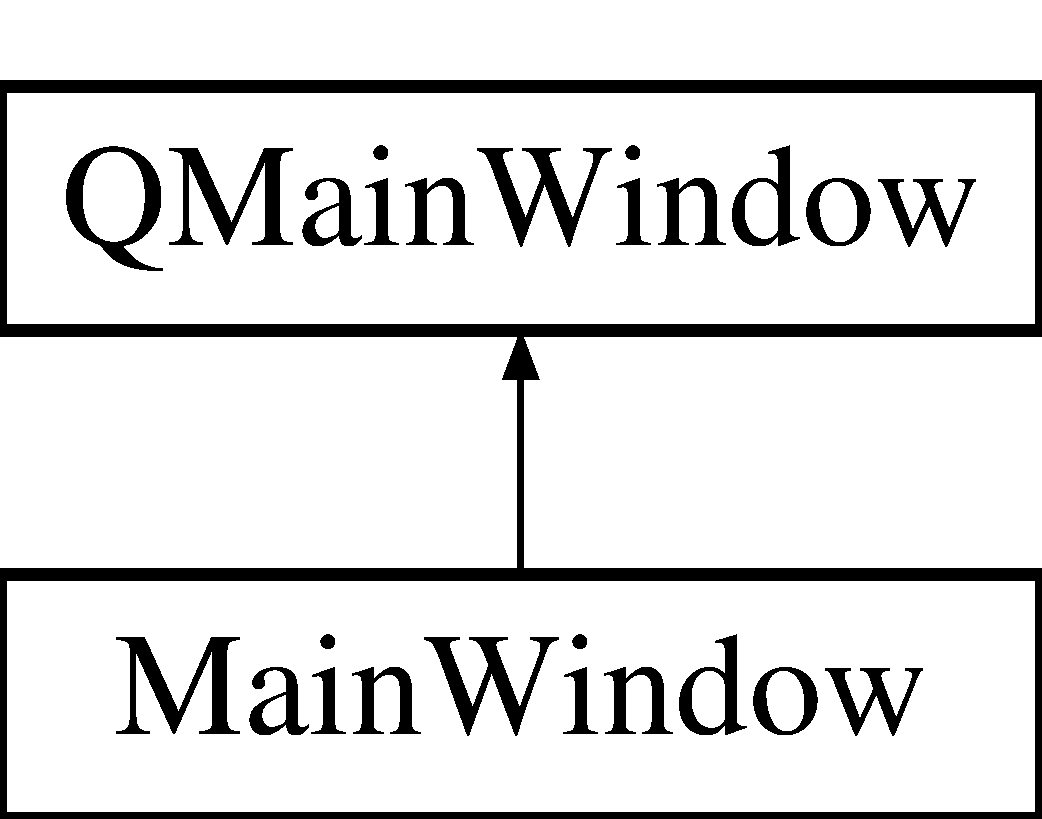
\includegraphics[height=2.000000cm]{class_main_window}
\end{center}
\end{figure}
\subsection*{Public Member Functions}
\begin{DoxyCompactItemize}
\item 
{\bfseries Main\+Window} (Q\+Widget $\ast$parent=0)\hypertarget{class_main_window_a8b244be8b7b7db1b08de2a2acb9409db}{}\label{class_main_window_a8b244be8b7b7db1b08de2a2acb9409db}

\end{DoxyCompactItemize}


The documentation for this class was generated from the following files\+:\begin{DoxyCompactItemize}
\item 
mainwindow.\+h\item 
mainwindow.\+cpp\end{DoxyCompactItemize}

\hypertarget{classmatrix}{}\section{matrix Class Reference}
\label{classmatrix}\index{matrix@{matrix}}


The matrix class une matrice constituer de vecteur de vecteur.  




{\ttfamily \#include $<$matrix.\+h$>$}

\subsection*{Public Member Functions}
\begin{DoxyCompactItemize}
\item 
\hyperlink{classmatrix_ac060122c49720709c23dd7e4e630eaff}{matrix} (int i, int j)
\begin{DoxyCompactList}\small\item\em matrix contrucreur matrice 2 d \end{DoxyCompactList}\item 
\hyperlink{classmatrix_afe22b82beac968bb2069201000e9b4bf}{matrix} (\hyperlink{classmatrix}{matrix} $\ast$obj)
\begin{DoxyCompactList}\small\item\em matrix constructeur par copie \end{DoxyCompactList}\item 
void \hyperlink{classmatrix_ab298b1344f474debfabd2db0e31e84c9}{set} (int x, int y)
\begin{DoxyCompactList}\small\item\em set met un 1 à la case de la matrice\{x\mbox{]}\mbox{[}y\mbox{]} \end{DoxyCompactList}\item 
void \hyperlink{classmatrix_ab039eefe55f3e60da940243505d20800}{afficher} ()\hypertarget{classmatrix_ab039eefe55f3e60da940243505d20800}{}\label{classmatrix_ab039eefe55f3e60da940243505d20800}

\begin{DoxyCompactList}\small\item\em afficher affiche la matrice \end{DoxyCompactList}\item 
void \hyperlink{classmatrix_a9b1fbe36a149d15a05cf43b1a2c01ee5}{resize\+Droite} ()\hypertarget{classmatrix_a9b1fbe36a149d15a05cf43b1a2c01ee5}{}\label{classmatrix_a9b1fbe36a149d15a05cf43b1a2c01ee5}

\begin{DoxyCompactList}\small\item\em resize\+Droite ajoute un vecteur remplie de 0 de taile size\+Row à droite \end{DoxyCompactList}\item 
void \hyperlink{classmatrix_a20b826143f701edefd8eacb92e44c7a6}{resize\+Gauche} ()\hypertarget{classmatrix_a20b826143f701edefd8eacb92e44c7a6}{}\label{classmatrix_a20b826143f701edefd8eacb92e44c7a6}

\begin{DoxyCompactList}\small\item\em resize\+Gauche ajoute un vecteur remplie de 0 de taile size\+Row à gauche \end{DoxyCompactList}\item 
bool \hyperlink{classmatrix_ab803b319d6488ae03985740b6437222f}{occuped} (int x, int y)
\begin{DoxyCompactList}\small\item\em occuped verifie si l\textquotesingle{}emplacement de la matrice\mbox{[}x\mbox{]}\mbox{[}y\mbox{]} est occupé \end{DoxyCompactList}\item 
void \hyperlink{classmatrix_a041925ba18b2fb25d350d0f6786d8a2a}{matrix\+To\+List} ()\hypertarget{classmatrix_a041925ba18b2fb25d350d0f6786d8a2a}{}\label{classmatrix_a041925ba18b2fb25d350d0f6786d8a2a}

\begin{DoxyCompactList}\small\item\em matrix\+To\+List convertie la matrice en afficga en liste de segment plein \end{DoxyCompactList}\item 
bool \hyperlink{classmatrix_ad1222d5c3689e27c2acd88fa1100b830}{vec\+Null} (vector$<$ int $>$ v)
\begin{DoxyCompactList}\small\item\em vec\+Null verifie si le vecteur v est remplie de 0 \end{DoxyCompactList}\item 
vector$<$ int $>$ \hyperlink{classmatrix_a83ac048f17c6031c31fd67242e37edc7}{vecteur\+To\+List} (vector$<$ int $>$ v)
\begin{DoxyCompactList}\small\item\em vecteur\+To\+List convertie un vecteir en un liste qui représente les segments pleins \end{DoxyCompactList}\item 
int \hyperlink{classmatrix_aa26916f337f663161fa8d1022919d41d}{calcul\+Offset} (vector$<$ int $>$ v1, vector$<$ int $>$ v2)
\begin{DoxyCompactList}\small\item\em calcul\+Offset calcule la différence de déplacement a faire entre v1 et v2 \end{DoxyCompactList}\item 
void \hyperlink{classmatrix_a56dd8532b44f9aed61b1f3b745d05a84}{printlist} ()\hypertarget{classmatrix_a56dd8532b44f9aed61b1f3b745d05a84}{}\label{classmatrix_a56dd8532b44f9aed61b1f3b745d05a84}

\begin{DoxyCompactList}\small\item\em printlist affiche la liste \end{DoxyCompactList}\item 
void \hyperlink{classmatrix_ab7e0ecebed1613e34a3cd81a3c5ad8b4}{propagation} (vector$<$ int $>$ $\ast$v, int i)
\begin{DoxyCompactList}\small\item\em propagation élimine les 1 consécutif dans les 2 sens du vecteur à l\textquotesingle{}indice i \end{DoxyCompactList}\item 
void \hyperlink{classmatrix_aba69eb1058b43b8690014fcbdf1764a6}{draw} (Q\+Painter \&painter, int x, int y, int sh, int sw)
\begin{DoxyCompactList}\small\item\em draw dessine le polyomino à partir de la matrice \end{DoxyCompactList}\end{DoxyCompactItemize}
\subsection*{Public Attributes}
\begin{DoxyCompactItemize}
\item 
int \hyperlink{classmatrix_accbce5e857edcccbc46f704db8d390a2}{size\+Row}\hypertarget{classmatrix_accbce5e857edcccbc46f704db8d390a2}{}\label{classmatrix_accbce5e857edcccbc46f704db8d390a2}

\begin{DoxyCompactList}\small\item\em size\+Row taille ligne \end{DoxyCompactList}\item 
int \hyperlink{classmatrix_a502f7b1bbd4aca8f56b562892aa7f550}{size\+Col}\hypertarget{classmatrix_a502f7b1bbd4aca8f56b562892aa7f550}{}\label{classmatrix_a502f7b1bbd4aca8f56b562892aa7f550}

\begin{DoxyCompactList}\small\item\em size\+Col taille colone \end{DoxyCompactList}\item 
vector$<$ vector$<$ int $>$ $>$ \hyperlink{classmatrix_a54bc336decc92a43de11b1b712af4e6a}{vec}\hypertarget{classmatrix_a54bc336decc92a43de11b1b712af4e6a}{}\label{classmatrix_a54bc336decc92a43de11b1b712af4e6a}

\begin{DoxyCompactList}\small\item\em vec l\textquotesingle{}architecture de la matrice \end{DoxyCompactList}\item 
vector$<$ vector$<$ int $>$ $>$ \hyperlink{classmatrix_a8a0bb1e77b1064c20a53aa51dea340a0}{l}\hypertarget{classmatrix_a8a0bb1e77b1064c20a53aa51dea340a0}{}\label{classmatrix_a8a0bb1e77b1064c20a53aa51dea340a0}

\begin{DoxyCompactList}\small\item\em l représente le polyomino sous forme de liste \end{DoxyCompactList}\end{DoxyCompactItemize}


\subsection{Detailed Description}
The matrix class une matrice constituer de vecteur de vecteur. 

\subsection{Constructor \& Destructor Documentation}
\index{matrix@{matrix}!matrix@{matrix}}
\index{matrix@{matrix}!matrix@{matrix}}
\subsubsection[{\texorpdfstring{matrix(int i, int j)}{matrix(int i, int j)}}]{\setlength{\rightskip}{0pt plus 5cm}matrix\+::matrix (
\begin{DoxyParamCaption}
\item[{int}]{i, }
\item[{int}]{j}
\end{DoxyParamCaption}
)}\hypertarget{classmatrix_ac060122c49720709c23dd7e4e630eaff}{}\label{classmatrix_ac060122c49720709c23dd7e4e630eaff}


matrix contrucreur matrice 2 d 


\begin{DoxyParams}{Parameters}
{\em i} & ligne \\
\hline
{\em j} & colone \\
\hline
\end{DoxyParams}
\index{matrix@{matrix}!matrix@{matrix}}
\index{matrix@{matrix}!matrix@{matrix}}
\subsubsection[{\texorpdfstring{matrix(matrix $\ast$obj)}{matrix(matrix *obj)}}]{\setlength{\rightskip}{0pt plus 5cm}matrix\+::matrix (
\begin{DoxyParamCaption}
\item[{{\bf matrix} $\ast$}]{obj}
\end{DoxyParamCaption}
)}\hypertarget{classmatrix_afe22b82beac968bb2069201000e9b4bf}{}\label{classmatrix_afe22b82beac968bb2069201000e9b4bf}


matrix constructeur par copie 


\begin{DoxyParams}{Parameters}
{\em obj} & \\
\hline
\end{DoxyParams}


\subsection{Member Function Documentation}
\index{matrix@{matrix}!calcul\+Offset@{calcul\+Offset}}
\index{calcul\+Offset@{calcul\+Offset}!matrix@{matrix}}
\subsubsection[{\texorpdfstring{calcul\+Offset(vector$<$ int $>$ v1, vector$<$ int $>$ v2)}{calculOffset(vector< int > v1, vector< int > v2)}}]{\setlength{\rightskip}{0pt plus 5cm}int matrix\+::calcul\+Offset (
\begin{DoxyParamCaption}
\item[{vector$<$ int $>$}]{v1, }
\item[{vector$<$ int $>$}]{v2}
\end{DoxyParamCaption}
)}\hypertarget{classmatrix_aa26916f337f663161fa8d1022919d41d}{}\label{classmatrix_aa26916f337f663161fa8d1022919d41d}


calcul\+Offset calcule la différence de déplacement a faire entre v1 et v2 


\begin{DoxyParams}{Parameters}
{\em v1} & \\
\hline
{\em v2} & \\
\hline
\end{DoxyParams}
\begin{DoxyReturn}{Returns}

\end{DoxyReturn}
\index{matrix@{matrix}!draw@{draw}}
\index{draw@{draw}!matrix@{matrix}}
\subsubsection[{\texorpdfstring{draw(\+Q\+Painter \&painter, int x, int y, int sh, int sw)}{draw(QPainter &painter, int x, int y, int sh, int sw)}}]{\setlength{\rightskip}{0pt plus 5cm}void matrix\+::draw (
\begin{DoxyParamCaption}
\item[{Q\+Painter \&}]{painter, }
\item[{int}]{x, }
\item[{int}]{y, }
\item[{int}]{sh, }
\item[{int}]{sw}
\end{DoxyParamCaption}
)}\hypertarget{classmatrix_aba69eb1058b43b8690014fcbdf1764a6}{}\label{classmatrix_aba69eb1058b43b8690014fcbdf1764a6}


draw dessine le polyomino à partir de la matrice 


\begin{DoxyParams}{Parameters}
{\em painter} & \\
\hline
{\em x} & \\
\hline
{\em y} & \\
\hline
{\em sh} & \\
\hline
{\em sw} & \\
\hline
\end{DoxyParams}
\index{matrix@{matrix}!occuped@{occuped}}
\index{occuped@{occuped}!matrix@{matrix}}
\subsubsection[{\texorpdfstring{occuped(int x, int y)}{occuped(int x, int y)}}]{\setlength{\rightskip}{0pt plus 5cm}bool matrix\+::occuped (
\begin{DoxyParamCaption}
\item[{int}]{x, }
\item[{int}]{y}
\end{DoxyParamCaption}
)}\hypertarget{classmatrix_ab803b319d6488ae03985740b6437222f}{}\label{classmatrix_ab803b319d6488ae03985740b6437222f}


occuped verifie si l\textquotesingle{}emplacement de la matrice\mbox{[}x\mbox{]}\mbox{[}y\mbox{]} est occupé 


\begin{DoxyParams}{Parameters}
{\em x} & \\
\hline
{\em y} & \\
\hline
\end{DoxyParams}
\begin{DoxyReturn}{Returns}

\end{DoxyReturn}
\index{matrix@{matrix}!propagation@{propagation}}
\index{propagation@{propagation}!matrix@{matrix}}
\subsubsection[{\texorpdfstring{propagation(vector$<$ int $>$ $\ast$v, int i)}{propagation(vector< int > *v, int i)}}]{\setlength{\rightskip}{0pt plus 5cm}void matrix\+::propagation (
\begin{DoxyParamCaption}
\item[{vector$<$ int $>$ $\ast$}]{v, }
\item[{int}]{i}
\end{DoxyParamCaption}
)}\hypertarget{classmatrix_ab7e0ecebed1613e34a3cd81a3c5ad8b4}{}\label{classmatrix_ab7e0ecebed1613e34a3cd81a3c5ad8b4}


propagation élimine les 1 consécutif dans les 2 sens du vecteur à l\textquotesingle{}indice i 


\begin{DoxyParams}{Parameters}
{\em v} & \\
\hline
{\em i} & \\
\hline
\end{DoxyParams}
\index{matrix@{matrix}!set@{set}}
\index{set@{set}!matrix@{matrix}}
\subsubsection[{\texorpdfstring{set(int x, int y)}{set(int x, int y)}}]{\setlength{\rightskip}{0pt plus 5cm}void matrix\+::set (
\begin{DoxyParamCaption}
\item[{int}]{x, }
\item[{int}]{y}
\end{DoxyParamCaption}
)}\hypertarget{classmatrix_ab298b1344f474debfabd2db0e31e84c9}{}\label{classmatrix_ab298b1344f474debfabd2db0e31e84c9}


set met un 1 à la case de la matrice\{x\mbox{]}\mbox{[}y\mbox{]} 


\begin{DoxyParams}{Parameters}
{\em x} & \\
\hline
{\em y} & \\
\hline
\end{DoxyParams}
\index{matrix@{matrix}!vec\+Null@{vec\+Null}}
\index{vec\+Null@{vec\+Null}!matrix@{matrix}}
\subsubsection[{\texorpdfstring{vec\+Null(vector$<$ int $>$ v)}{vecNull(vector< int > v)}}]{\setlength{\rightskip}{0pt plus 5cm}bool matrix\+::vec\+Null (
\begin{DoxyParamCaption}
\item[{vector$<$ int $>$}]{v}
\end{DoxyParamCaption}
)}\hypertarget{classmatrix_ad1222d5c3689e27c2acd88fa1100b830}{}\label{classmatrix_ad1222d5c3689e27c2acd88fa1100b830}


vec\+Null verifie si le vecteur v est remplie de 0 


\begin{DoxyParams}{Parameters}
{\em v} & \\
\hline
\end{DoxyParams}
\begin{DoxyReturn}{Returns}

\end{DoxyReturn}
\index{matrix@{matrix}!vecteur\+To\+List@{vecteur\+To\+List}}
\index{vecteur\+To\+List@{vecteur\+To\+List}!matrix@{matrix}}
\subsubsection[{\texorpdfstring{vecteur\+To\+List(vector$<$ int $>$ v)}{vecteurToList(vector< int > v)}}]{\setlength{\rightskip}{0pt plus 5cm}vector$<$ int $>$ matrix\+::vecteur\+To\+List (
\begin{DoxyParamCaption}
\item[{vector$<$ int $>$}]{v}
\end{DoxyParamCaption}
)}\hypertarget{classmatrix_a83ac048f17c6031c31fd67242e37edc7}{}\label{classmatrix_a83ac048f17c6031c31fd67242e37edc7}


vecteur\+To\+List convertie un vecteir en un liste qui représente les segments pleins 


\begin{DoxyParams}{Parameters}
{\em v} & \\
\hline
\end{DoxyParams}
\begin{DoxyReturn}{Returns}

\end{DoxyReturn}


The documentation for this class was generated from the following files\+:\begin{DoxyCompactItemize}
\item 
\hyperlink{matrix_8h}{matrix.\+h}\item 
\hyperlink{matrix_8cpp}{matrix.\+cpp}\end{DoxyCompactItemize}

\hypertarget{class_segment}{}\section{Segment Class Reference}
\label{class_segment}\index{Segment@{Segment}}


The \hyperlink{class_segment}{Segment} class Représente un liste d\textquotesingle{}unicell.  




{\ttfamily \#include $<$segment.\+h$>$}

\subsection*{Public Member Functions}
\begin{DoxyCompactItemize}
\item 
\hyperlink{class_segment_a8251e7e03f8fb4a65a35f1c7a1c6e806}{Segment} (int x, int y, int area, bool f)
\begin{DoxyCompactList}\small\item\em \hyperlink{class_segment}{Segment} constructeur. \end{DoxyCompactList}\item 
void \hyperlink{class_segment_ad3d691fcf0dd3e1c6478274589cfb425}{draw} (Q\+Painter \&painter, int x, int y, int sh, int sw)
\begin{DoxyCompactList}\small\item\em draw dessine une par une les unitcells \end{DoxyCompactList}\item 
void \hyperlink{class_segment_afac9424a18e0e264208d754cc3a1439a}{rotate} ()\hypertarget{class_segment_afac9424a18e0e264208d754cc3a1439a}{}\label{class_segment_afac9424a18e0e264208d754cc3a1439a}

\begin{DoxyCompactList}\small\item\em rotate permet la rotation d\textquotesingle{}un segment à 90dégrès \end{DoxyCompactList}\item 
\hyperlink{class_unit_cell}{Unit\+Cell} $\ast$ \hyperlink{class_segment_a4c02741758eaae91a7e5fe04ea33aa17}{get\+Unit\+Cell} (int index)
\begin{DoxyCompactList}\small\item\em get\+Unit\+Cell renvoie l\textquotesingle{}unitcell à l\textquotesingle{}index indiqué \end{DoxyCompactList}\item 
vector$<$ \hyperlink{class_unit_cell}{Unit\+Cell} $>$ $\ast$ \hyperlink{class_segment_a65060dd0d9d490054056869caea68a44}{get\+Cells} ()
\begin{DoxyCompactList}\small\item\em get\+Cells renvoie toutes les unitcells \end{DoxyCompactList}\item 
int \hyperlink{class_segment_a96c4597d9f2265ca8a11604562627888}{get\+Size} () const 
\begin{DoxyCompactList}\small\item\em get\+Size renvoie la taille \end{DoxyCompactList}\item 
bool \hyperlink{class_segment_a85de0a9a7b0e1bb9e7397b147a19f959}{is\+Down} ()
\begin{DoxyCompactList}\small\item\em is\+Down verifie sur le segment est placé \end{DoxyCompactList}\item 
bool \hyperlink{class_segment_af810a0fcfc2a5e412237777433906eba}{neighbor} (\hyperlink{class_segment}{Segment} $\ast$other)
\begin{DoxyCompactList}\small\item\em neighbor \end{DoxyCompactList}\item 
void \hyperlink{class_segment_ab51341d5b76009abb2ac69f870fb2633}{reset} (int x)
\begin{DoxyCompactList}\small\item\em reset verifie si 2 segments sont voisin \end{DoxyCompactList}\end{DoxyCompactItemize}
\subsection*{Public Attributes}
\begin{DoxyCompactItemize}
\item 
vector$<$ \hyperlink{class_unit_cell}{Unit\+Cell} $>$ \hyperlink{class_segment_a931b5815778e37b4906f9c079432c5db}{cells}\hypertarget{class_segment_a931b5815778e37b4906f9c079432c5db}{}\label{class_segment_a931b5815778e37b4906f9c079432c5db}

\begin{DoxyCompactList}\small\item\em cells toutes les \hyperlink{class_unit_cell}{Unit\+Cell} qui constitue le segment \end{DoxyCompactList}\item 
bool \hyperlink{class_segment_a64effb3c704066934c7bfb3d5f76dead}{verticale}\hypertarget{class_segment_a64effb3c704066934c7bfb3d5f76dead}{}\label{class_segment_a64effb3c704066934c7bfb3d5f76dead}

\begin{DoxyCompactList}\small\item\em verticale true si horizontale \end{DoxyCompactList}\item 
Q\+Color \hyperlink{class_segment_ae17457fa5c481d65fa0bd6363069e144}{color}\hypertarget{class_segment_ae17457fa5c481d65fa0bd6363069e144}{}\label{class_segment_ae17457fa5c481d65fa0bd6363069e144}

\begin{DoxyCompactList}\small\item\em color couleur du segment \end{DoxyCompactList}\end{DoxyCompactItemize}


\subsection{Detailed Description}
The \hyperlink{class_segment}{Segment} class Représente un liste d\textquotesingle{}unicell. 

\subsection{Constructor \& Destructor Documentation}
\index{Segment@{Segment}!Segment@{Segment}}
\index{Segment@{Segment}!Segment@{Segment}}
\subsubsection[{\texorpdfstring{Segment(int x, int y, int area, bool f)}{Segment(int x, int y, int area, bool f)}}]{\setlength{\rightskip}{0pt plus 5cm}Segment\+::\+Segment (
\begin{DoxyParamCaption}
\item[{int}]{x, }
\item[{int}]{y, }
\item[{int}]{area, }
\item[{bool}]{f}
\end{DoxyParamCaption}
)}\hypertarget{class_segment_a8251e7e03f8fb4a65a35f1c7a1c6e806}{}\label{class_segment_a8251e7e03f8fb4a65a35f1c7a1c6e806}


\hyperlink{class_segment}{Segment} constructeur. 


\begin{DoxyParams}{Parameters}
{\em x} & coordonée de départ du segment \\
\hline
{\em y} & coordonée de départ du segment \\
\hline
{\em area} & sa taille \\
\hline
{\em f} & sa position true si horizontale \\
\hline
\end{DoxyParams}


\subsection{Member Function Documentation}
\index{Segment@{Segment}!draw@{draw}}
\index{draw@{draw}!Segment@{Segment}}
\subsubsection[{\texorpdfstring{draw(\+Q\+Painter \&painter, int x, int y, int sh, int sw)}{draw(QPainter &painter, int x, int y, int sh, int sw)}}]{\setlength{\rightskip}{0pt plus 5cm}void Segment\+::draw (
\begin{DoxyParamCaption}
\item[{Q\+Painter \&}]{painter, }
\item[{int}]{x, }
\item[{int}]{y, }
\item[{int}]{sh, }
\item[{int}]{sw}
\end{DoxyParamCaption}
)}\hypertarget{class_segment_ad3d691fcf0dd3e1c6478274589cfb425}{}\label{class_segment_ad3d691fcf0dd3e1c6478274589cfb425}


draw dessine une par une les unitcells 


\begin{DoxyParams}{Parameters}
{\em painter} & \\
\hline
{\em x} & \\
\hline
{\em y} & \\
\hline
{\em sh} & \\
\hline
{\em sw} & \\
\hline
\end{DoxyParams}
\index{Segment@{Segment}!get\+Cells@{get\+Cells}}
\index{get\+Cells@{get\+Cells}!Segment@{Segment}}
\subsubsection[{\texorpdfstring{get\+Cells()}{getCells()}}]{\setlength{\rightskip}{0pt plus 5cm}vector$<${\bf Unit\+Cell}$>$$\ast$ Segment\+::get\+Cells (
\begin{DoxyParamCaption}
{}
\end{DoxyParamCaption}
)\hspace{0.3cm}{\ttfamily [inline]}}\hypertarget{class_segment_a65060dd0d9d490054056869caea68a44}{}\label{class_segment_a65060dd0d9d490054056869caea68a44}


get\+Cells renvoie toutes les unitcells 

\begin{DoxyReturn}{Returns}

\end{DoxyReturn}
\index{Segment@{Segment}!get\+Size@{get\+Size}}
\index{get\+Size@{get\+Size}!Segment@{Segment}}
\subsubsection[{\texorpdfstring{get\+Size() const }{getSize() const }}]{\setlength{\rightskip}{0pt plus 5cm}int Segment\+::get\+Size (
\begin{DoxyParamCaption}
{}
\end{DoxyParamCaption}
) const\hspace{0.3cm}{\ttfamily [inline]}}\hypertarget{class_segment_a96c4597d9f2265ca8a11604562627888}{}\label{class_segment_a96c4597d9f2265ca8a11604562627888}


get\+Size renvoie la taille 

\begin{DoxyReturn}{Returns}

\end{DoxyReturn}
\index{Segment@{Segment}!get\+Unit\+Cell@{get\+Unit\+Cell}}
\index{get\+Unit\+Cell@{get\+Unit\+Cell}!Segment@{Segment}}
\subsubsection[{\texorpdfstring{get\+Unit\+Cell(int index)}{getUnitCell(int index)}}]{\setlength{\rightskip}{0pt plus 5cm}{\bf Unit\+Cell}$\ast$ Segment\+::get\+Unit\+Cell (
\begin{DoxyParamCaption}
\item[{int}]{index}
\end{DoxyParamCaption}
)\hspace{0.3cm}{\ttfamily [inline]}}\hypertarget{class_segment_a4c02741758eaae91a7e5fe04ea33aa17}{}\label{class_segment_a4c02741758eaae91a7e5fe04ea33aa17}


get\+Unit\+Cell renvoie l\textquotesingle{}unitcell à l\textquotesingle{}index indiqué 


\begin{DoxyParams}{Parameters}
{\em index} & \\
\hline
\end{DoxyParams}
\begin{DoxyReturn}{Returns}

\end{DoxyReturn}
\index{Segment@{Segment}!is\+Down@{is\+Down}}
\index{is\+Down@{is\+Down}!Segment@{Segment}}
\subsubsection[{\texorpdfstring{is\+Down()}{isDown()}}]{\setlength{\rightskip}{0pt plus 5cm}bool Segment\+::is\+Down (
\begin{DoxyParamCaption}
{}
\end{DoxyParamCaption}
)}\hypertarget{class_segment_a85de0a9a7b0e1bb9e7397b147a19f959}{}\label{class_segment_a85de0a9a7b0e1bb9e7397b147a19f959}


is\+Down verifie sur le segment est placé 

\begin{DoxyReturn}{Returns}

\end{DoxyReturn}
\index{Segment@{Segment}!neighbor@{neighbor}}
\index{neighbor@{neighbor}!Segment@{Segment}}
\subsubsection[{\texorpdfstring{neighbor(\+Segment $\ast$other)}{neighbor(Segment *other)}}]{\setlength{\rightskip}{0pt plus 5cm}bool Segment\+::neighbor (
\begin{DoxyParamCaption}
\item[{{\bf Segment} $\ast$}]{other}
\end{DoxyParamCaption}
)}\hypertarget{class_segment_af810a0fcfc2a5e412237777433906eba}{}\label{class_segment_af810a0fcfc2a5e412237777433906eba}


neighbor 


\begin{DoxyParams}{Parameters}
{\em other} & \\
\hline
\end{DoxyParams}
\begin{DoxyReturn}{Returns}

\end{DoxyReturn}
\index{Segment@{Segment}!reset@{reset}}
\index{reset@{reset}!Segment@{Segment}}
\subsubsection[{\texorpdfstring{reset(int x)}{reset(int x)}}]{\setlength{\rightskip}{0pt plus 5cm}void Segment\+::reset (
\begin{DoxyParamCaption}
\item[{int}]{x}
\end{DoxyParamCaption}
)}\hypertarget{class_segment_ab51341d5b76009abb2ac69f870fb2633}{}\label{class_segment_ab51341d5b76009abb2ac69f870fb2633}


reset verifie si 2 segments sont voisin 


\begin{DoxyParams}{Parameters}
{\em x} & reset remet un segment à ses coordonées d\textquotesingle{}origine \\
\hline
{\em x} & \\
\hline
\end{DoxyParams}


The documentation for this class was generated from the following files\+:\begin{DoxyCompactItemize}
\item 
\hyperlink{segment_8h}{segment.\+h}\item 
\hyperlink{segment_8cpp}{segment.\+cpp}\end{DoxyCompactItemize}

\hypertarget{class_unit_cell}{}\section{Unit\+Cell Class Reference}
\label{class_unit_cell}\index{Unit\+Cell@{Unit\+Cell}}


The \hyperlink{class_unit_cell}{Unit\+Cell} class contient la taille ,la couleur,et les coordonées d\textquotesingle{}une celluled\textquotesingle{}un polyomino.  




{\ttfamily \#include $<$unitcell.\+h$>$}

\subsection*{Public Member Functions}
\begin{DoxyCompactItemize}
\item 
\hyperlink{class_unit_cell_a5dbf3b36af02e1ea1957c93b79ba8099}{Unit\+Cell} (int \hyperlink{class_unit_cell_aae64c4e864e786746eba53443f946d69}{x}, int \hyperlink{class_unit_cell_a9fdd4a78e21c23d47e535ed2510002ad}{y}, Q\+Color \hyperlink{class_unit_cell_a6e7907cda650addf06f7f06c690180de}{color})
\begin{DoxyCompactList}\small\item\em \hyperlink{class_unit_cell}{Unit\+Cell} constructeur. \end{DoxyCompactList}\item 
void \hyperlink{class_unit_cell_a903afaf6948b87afd78cc971674b60cd}{draw} (Q\+Painter \&painter, int \hyperlink{class_unit_cell_aae64c4e864e786746eba53443f946d69}{x}, int \hyperlink{class_unit_cell_a9fdd4a78e21c23d47e535ed2510002ad}{y}, int sh, int sw)
\begin{DoxyCompactList}\small\item\em draw dessine une cellule de polyomino \end{DoxyCompactList}\end{DoxyCompactItemize}
\subsection*{Static Public Member Functions}
\begin{DoxyCompactItemize}
\item 
static void \hyperlink{class_unit_cell_a30d1461d8760fb72d87f683811df0d4e}{set\+Size} (int \hyperlink{class_unit_cell_ab90b8bcef203bb8a7341bf2b11aa48ac}{h}, int \hyperlink{class_unit_cell_a36cb2e967f43f4e71ded533752a92a1c}{w})
\begin{DoxyCompactList}\small\item\em set\+Size change la hauteur et la largeur \end{DoxyCompactList}\item 
static int \hyperlink{class_unit_cell_af42b23a4f6689ee4bfcdc43454ea2a4e}{get\+Height} ()
\begin{DoxyCompactList}\small\item\em get\+Height accesseur de la hauteur \end{DoxyCompactList}\item 
static int \hyperlink{class_unit_cell_a151f78bd5616f3e554c3e19077b96fb7}{get\+Width} ()
\begin{DoxyCompactList}\small\item\em get\+Width accesseur de la largeur \end{DoxyCompactList}\end{DoxyCompactItemize}
\subsection*{Public Attributes}
\begin{DoxyCompactItemize}
\item 
int \hyperlink{class_unit_cell_aae64c4e864e786746eba53443f946d69}{x} = 0\hypertarget{class_unit_cell_aae64c4e864e786746eba53443f946d69}{}\label{class_unit_cell_aae64c4e864e786746eba53443f946d69}

\begin{DoxyCompactList}\small\item\em x coordonés abscisse \end{DoxyCompactList}\item 
int \hyperlink{class_unit_cell_a9fdd4a78e21c23d47e535ed2510002ad}{y} = 0\hypertarget{class_unit_cell_a9fdd4a78e21c23d47e535ed2510002ad}{}\label{class_unit_cell_a9fdd4a78e21c23d47e535ed2510002ad}

\begin{DoxyCompactList}\small\item\em y coordonés ordonné \end{DoxyCompactList}\item 
Q\+Color \hyperlink{class_unit_cell_a6e7907cda650addf06f7f06c690180de}{color}\hypertarget{class_unit_cell_a6e7907cda650addf06f7f06c690180de}{}\label{class_unit_cell_a6e7907cda650addf06f7f06c690180de}

\begin{DoxyCompactList}\small\item\em color couleur \end{DoxyCompactList}\end{DoxyCompactItemize}
\subsection*{Static Protected Attributes}
\begin{DoxyCompactItemize}
\item 
static int \hyperlink{class_unit_cell_ab90b8bcef203bb8a7341bf2b11aa48ac}{h} = 0\hypertarget{class_unit_cell_ab90b8bcef203bb8a7341bf2b11aa48ac}{}\label{class_unit_cell_ab90b8bcef203bb8a7341bf2b11aa48ac}

\begin{DoxyCompactList}\small\item\em h sa hauteur \end{DoxyCompactList}\item 
static int \hyperlink{class_unit_cell_a36cb2e967f43f4e71ded533752a92a1c}{w} = 0\hypertarget{class_unit_cell_a36cb2e967f43f4e71ded533752a92a1c}{}\label{class_unit_cell_a36cb2e967f43f4e71ded533752a92a1c}

\begin{DoxyCompactList}\small\item\em w sa largeur \end{DoxyCompactList}\end{DoxyCompactItemize}


\subsection{Detailed Description}
The \hyperlink{class_unit_cell}{Unit\+Cell} class contient la taille ,la couleur,et les coordonées d\textquotesingle{}une celluled\textquotesingle{}un polyomino. 

\subsection{Constructor \& Destructor Documentation}
\index{Unit\+Cell@{Unit\+Cell}!Unit\+Cell@{Unit\+Cell}}
\index{Unit\+Cell@{Unit\+Cell}!Unit\+Cell@{Unit\+Cell}}
\subsubsection[{\texorpdfstring{Unit\+Cell(int x, int y, Q\+Color color)}{UnitCell(int x, int y, QColor color)}}]{\setlength{\rightskip}{0pt plus 5cm}Unit\+Cell\+::\+Unit\+Cell (
\begin{DoxyParamCaption}
\item[{int}]{x, }
\item[{int}]{y, }
\item[{Q\+Color}]{color}
\end{DoxyParamCaption}
)}\hypertarget{class_unit_cell_a5dbf3b36af02e1ea1957c93b79ba8099}{}\label{class_unit_cell_a5dbf3b36af02e1ea1957c93b79ba8099}


\hyperlink{class_unit_cell}{Unit\+Cell} constructeur. 


\begin{DoxyParams}{Parameters}
{\em x} & \\
\hline
{\em y} & \\
\hline
{\em color} & \\
\hline
\end{DoxyParams}


\subsection{Member Function Documentation}
\index{Unit\+Cell@{Unit\+Cell}!draw@{draw}}
\index{draw@{draw}!Unit\+Cell@{Unit\+Cell}}
\subsubsection[{\texorpdfstring{draw(\+Q\+Painter \&painter, int x, int y, int sh, int sw)}{draw(QPainter &painter, int x, int y, int sh, int sw)}}]{\setlength{\rightskip}{0pt plus 5cm}void Unit\+Cell\+::draw (
\begin{DoxyParamCaption}
\item[{Q\+Painter \&}]{painter, }
\item[{int}]{x, }
\item[{int}]{y, }
\item[{int}]{sh, }
\item[{int}]{sw}
\end{DoxyParamCaption}
)}\hypertarget{class_unit_cell_a903afaf6948b87afd78cc971674b60cd}{}\label{class_unit_cell_a903afaf6948b87afd78cc971674b60cd}


draw dessine une cellule de polyomino 


\begin{DoxyParams}{Parameters}
{\em painter} & \\
\hline
{\em x} & \\
\hline
{\em y} & \\
\hline
{\em sh} & \\
\hline
{\em sw} & \\
\hline
\end{DoxyParams}
\index{Unit\+Cell@{Unit\+Cell}!get\+Height@{get\+Height}}
\index{get\+Height@{get\+Height}!Unit\+Cell@{Unit\+Cell}}
\subsubsection[{\texorpdfstring{get\+Height()}{getHeight()}}]{\setlength{\rightskip}{0pt plus 5cm}int Unit\+Cell\+::get\+Height (
\begin{DoxyParamCaption}
{}
\end{DoxyParamCaption}
)\hspace{0.3cm}{\ttfamily [static]}}\hypertarget{class_unit_cell_af42b23a4f6689ee4bfcdc43454ea2a4e}{}\label{class_unit_cell_af42b23a4f6689ee4bfcdc43454ea2a4e}


get\+Height accesseur de la hauteur 

\begin{DoxyReturn}{Returns}

\end{DoxyReturn}
\index{Unit\+Cell@{Unit\+Cell}!get\+Width@{get\+Width}}
\index{get\+Width@{get\+Width}!Unit\+Cell@{Unit\+Cell}}
\subsubsection[{\texorpdfstring{get\+Width()}{getWidth()}}]{\setlength{\rightskip}{0pt plus 5cm}int Unit\+Cell\+::get\+Width (
\begin{DoxyParamCaption}
{}
\end{DoxyParamCaption}
)\hspace{0.3cm}{\ttfamily [static]}}\hypertarget{class_unit_cell_a151f78bd5616f3e554c3e19077b96fb7}{}\label{class_unit_cell_a151f78bd5616f3e554c3e19077b96fb7}


get\+Width accesseur de la largeur 

\begin{DoxyReturn}{Returns}

\end{DoxyReturn}
\index{Unit\+Cell@{Unit\+Cell}!set\+Size@{set\+Size}}
\index{set\+Size@{set\+Size}!Unit\+Cell@{Unit\+Cell}}
\subsubsection[{\texorpdfstring{set\+Size(int h, int w)}{setSize(int h, int w)}}]{\setlength{\rightskip}{0pt plus 5cm}void Unit\+Cell\+::set\+Size (
\begin{DoxyParamCaption}
\item[{int}]{h, }
\item[{int}]{w}
\end{DoxyParamCaption}
)\hspace{0.3cm}{\ttfamily [static]}}\hypertarget{class_unit_cell_a30d1461d8760fb72d87f683811df0d4e}{}\label{class_unit_cell_a30d1461d8760fb72d87f683811df0d4e}


set\+Size change la hauteur et la largeur 


\begin{DoxyParams}{Parameters}
{\em h} & \\
\hline
{\em w} & \\
\hline
\end{DoxyParams}


The documentation for this class was generated from the following files\+:\begin{DoxyCompactItemize}
\item 
\hyperlink{unitcell_8h}{unitcell.\+h}\item 
\hyperlink{unitcell_8cpp}{unitcell.\+cpp}\end{DoxyCompactItemize}

\hypertarget{class_window}{}\section{Window Class Reference}
\label{class_window}\index{Window@{Window}}


The \hyperlink{class_window}{Window} class contient tous les widgets de l\textquotesingle{}application.  




{\ttfamily \#include $<$window.\+h$>$}

Inheritance diagram for Window\+:\begin{figure}[H]
\begin{center}
\leavevmode
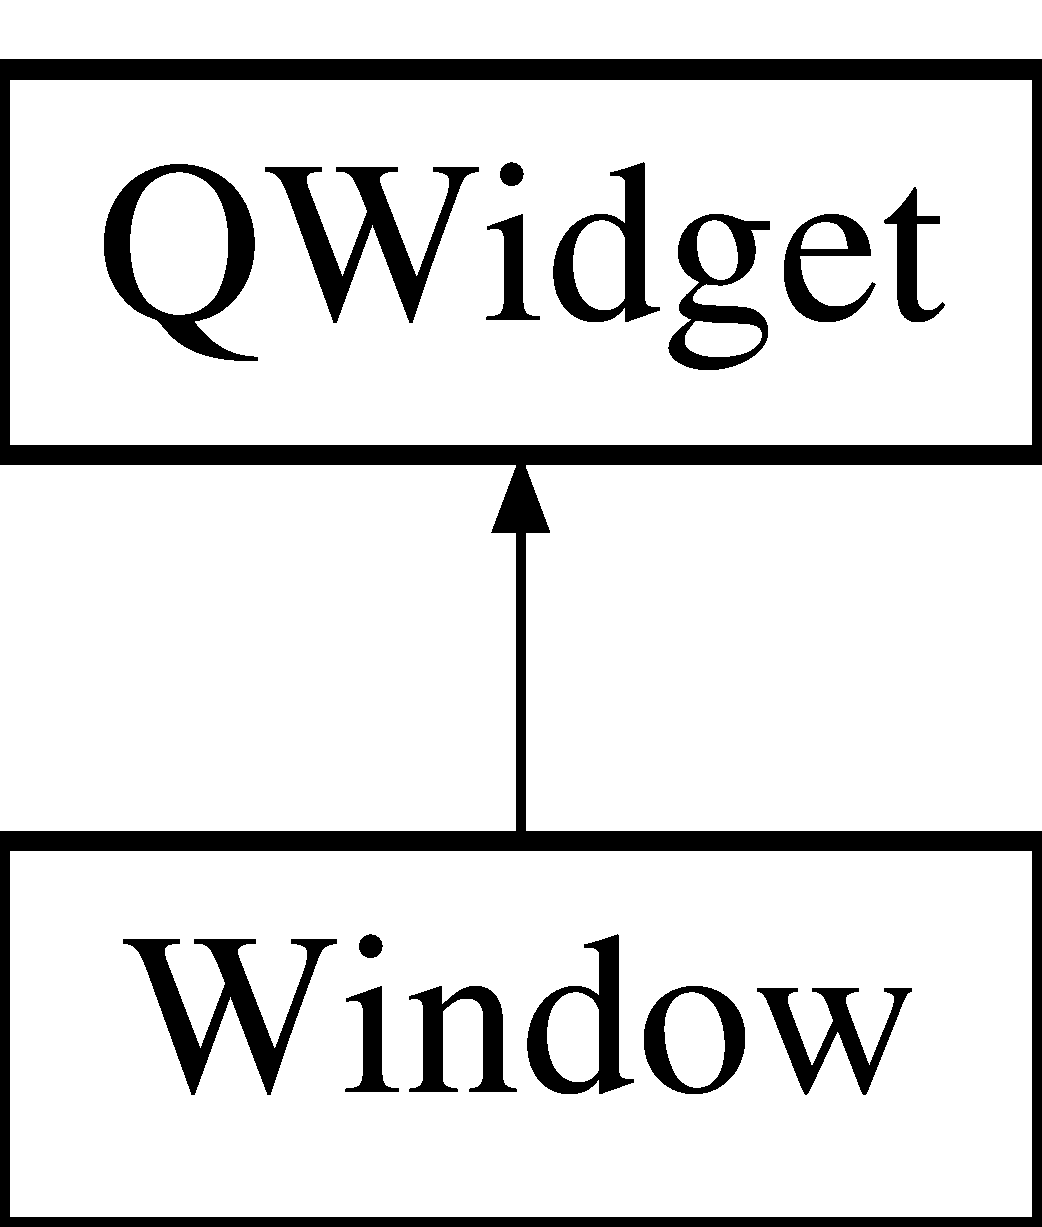
\includegraphics[height=2.000000cm]{class_window}
\end{center}
\end{figure}
\subsection*{Public Slots}
\begin{DoxyCompactItemize}
\item 
void \hyperlink{class_window_a5cddf5e150455180e95f8419a52dd380}{switch\+Start\+Restart\+Btn} ()\hypertarget{class_window_a5cddf5e150455180e95f8419a52dd380}{}\label{class_window_a5cddf5e150455180e95f8419a52dd380}

\begin{DoxyCompactList}\small\item\em switch\+Start\+Restart\+Btn permet de lier le bouton start de l\textquotesingle{}apply et la fonction board\+::start(). \end{DoxyCompactList}\item 
void \hyperlink{class_window_ad57b8f4814d9dba8bb23d60ca256f328}{switch\+Pause\+Play\+Btn} ()\hypertarget{class_window_ad57b8f4814d9dba8bb23d60ca256f328}{}\label{class_window_ad57b8f4814d9dba8bb23d60ca256f328}

\begin{DoxyCompactList}\small\item\em switch\+Pause\+Play\+Btn permet de lier le bouton start de l\textquotesingle{}apply et la fonction board\+::pause(). \end{DoxyCompactList}\item 
void {\bfseries switchB} ()\hypertarget{class_window_a5d60708e4577aff4fa1c932971963b06}{}\label{class_window_a5d60708e4577aff4fa1c932971963b06}

\end{DoxyCompactItemize}
\subsection*{Public Member Functions}
\begin{DoxyCompactItemize}
\item 
\hyperlink{class_window_a74e6087da23d3c24e9fac0245e5ec92c}{Window} ()\hypertarget{class_window_a74e6087da23d3c24e9fac0245e5ec92c}{}\label{class_window_a74e6087da23d3c24e9fac0245e5ec92c}

\begin{DoxyCompactList}\small\item\em \hyperlink{class_window}{Window} constructeur. \end{DoxyCompactList}\end{DoxyCompactItemize}
\subsection*{Public Attributes}
\begin{DoxyCompactItemize}
\item 
\hyperlink{class_board}{Board} $\ast$ \hyperlink{class_window_a906c0c4c45bc154db38b36550596aeb2}{boardT}\hypertarget{class_window_a906c0c4c45bc154db38b36550596aeb2}{}\label{class_window_a906c0c4c45bc154db38b36550596aeb2}

\begin{DoxyCompactList}\small\item\em board le widget ou l\textquotesingle{}on dessine \end{DoxyCompactList}\item 
\hyperlink{class_board2}{Board2} $\ast$ \hyperlink{class_window_aa11d094243940ed58d7ac5506efe2707}{boardV}\hypertarget{class_window_aa11d094243940ed58d7ac5506efe2707}{}\label{class_window_aa11d094243940ed58d7ac5506efe2707}

\begin{DoxyCompactList}\small\item\em board2 \end{DoxyCompactList}\item 
Q\+Label $\ast$ \hyperlink{class_window_a5f4fdd6881f2b071bad324bc0e01ab36}{label}\hypertarget{class_window_a5f4fdd6881f2b071bad324bc0e01ab36}{}\label{class_window_a5f4fdd6881f2b071bad324bc0e01ab36}

\begin{DoxyCompactList}\small\item\em label nom de widget \end{DoxyCompactList}\item 
Q\+Push\+Button $\ast$ \hyperlink{class_window_a3005a3efaf6600a44b879b7d0f36fecd}{start\+Btn}\hypertarget{class_window_a3005a3efaf6600a44b879b7d0f36fecd}{}\label{class_window_a3005a3efaf6600a44b879b7d0f36fecd}

\begin{DoxyCompactList}\small\item\em start\+Btn bouton start \end{DoxyCompactList}\item 
Q\+Push\+Button $\ast$ \hyperlink{class_window_a874073f85555346739380a5c21892553}{pause\+Btn}\hypertarget{class_window_a874073f85555346739380a5c21892553}{}\label{class_window_a874073f85555346739380a5c21892553}

\begin{DoxyCompactList}\small\item\em pause\+Btn bouton pause \end{DoxyCompactList}\item 
Q\+Push\+Button $\ast$ \hyperlink{class_window_a2b98fdaee75065f48ce1694cb42a616a}{quit\+Btn}\hypertarget{class_window_a2b98fdaee75065f48ce1694cb42a616a}{}\label{class_window_a2b98fdaee75065f48ce1694cb42a616a}

\begin{DoxyCompactList}\small\item\em quit\+Btn bouton quit \end{DoxyCompactList}\item 
Q\+L\+C\+D\+Number $\ast$ \hyperlink{class_window_a35b1d4ab7d60ceff7daa5d817314226c}{surface\+Lcd}\hypertarget{class_window_a35b1d4ab7d60ceff7daa5d817314226c}{}\label{class_window_a35b1d4ab7d60ceff7daa5d817314226c}

\begin{DoxyCompactList}\small\item\em surface\+Lcd affichage du score \end{DoxyCompactList}\item 
Q\+Push\+Button $\ast$ \hyperlink{class_window_af958997387b1124f1bf2b47b7230db74}{switch\+Btn}\hypertarget{class_window_af958997387b1124f1bf2b47b7230db74}{}\label{class_window_af958997387b1124f1bf2b47b7230db74}

\begin{DoxyCompactList}\small\item\em switch\+Btn switch pour passer en mode visualisation de polyominos \end{DoxyCompactList}\item 
bool {\bfseries switch\+Visu} =false\hypertarget{class_window_aeb85a2399e59772014289c10440d401a}{}\label{class_window_aeb85a2399e59772014289c10440d401a}

\end{DoxyCompactItemize}


\subsection{Detailed Description}
The \hyperlink{class_window}{Window} class contient tous les widgets de l\textquotesingle{}application. 

The documentation for this class was generated from the following files\+:\begin{DoxyCompactItemize}
\item 
\hyperlink{window_8h}{window.\+h}\item 
\hyperlink{window_8cpp}{window.\+cpp}\end{DoxyCompactItemize}

\chapter{File Documentation}
\hypertarget{board_8cpp}{}\section{board.\+cpp File Reference}
\label{board_8cpp}\index{board.\+cpp@{board.\+cpp}}


gestion de la partie.  


{\ttfamily \#include $<$iostream$>$}\\*
{\ttfamily \#include $<$time.\+h$>$}\\*
{\ttfamily \#include \char`\"{}Board.\+h\char`\"{}}\\*
{\ttfamily \#include $<$Q\+Key\+Event$>$}\\*
{\ttfamily \#include $<$fstream$>$}\\*


\subsection{Detailed Description}
gestion de la partie. 

\begin{DoxyAuthor}{Author}
Fagard.\+C 
\end{DoxyAuthor}
\begin{DoxyVersion}{Version}
0.\+1 
\end{DoxyVersion}
\begin{DoxyDate}{Date}
14juin 2016
\end{DoxyDate}
Moteur du jeu 
\hypertarget{board_8h}{}\section{board.\+h File Reference}
\label{board_8h}\index{board.\+h@{board.\+h}}


gestion de la partie.  


{\ttfamily \#include $<$Q\+Frame$>$}\\*
{\ttfamily \#include $<$Q\+Basic\+Timer$>$}\\*
{\ttfamily \#include $<$Q\+Timer\+Event$>$}\\*
{\ttfamily \#include \char`\"{}Unit\+Cell.\+h\char`\"{}}\\*
{\ttfamily \#include \char`\"{}Segment.\+h\char`\"{}}\\*
{\ttfamily \#include \char`\"{}matrix.\+h\char`\"{}}\\*
\subsection*{Classes}
\begin{DoxyCompactItemize}
\item 
class \hyperlink{class_board}{Board}
\begin{DoxyCompactList}\small\item\em classe representant le lecteur \end{DoxyCompactList}\end{DoxyCompactItemize}
\subsection*{Enumerations}
\begin{DoxyCompactItemize}
\item 
enum \{ {\bfseries M\+O\+V\+E\+\_\+\+D\+O\+WN}, 
{\bfseries M\+O\+V\+E\+\_\+\+L\+E\+FT}, 
{\bfseries M\+O\+V\+E\+\_\+\+R\+I\+G\+HT}
 \}\hypertarget{board_8h_a06fc87d81c62e9abb8790b6e5713c55b}{}\label{board_8h_a06fc87d81c62e9abb8790b6e5713c55b}

\end{DoxyCompactItemize}


\subsection{Detailed Description}
gestion de la partie. 

\begin{DoxyAuthor}{Author}
Fagard.\+C 
\end{DoxyAuthor}
\begin{DoxyVersion}{Version}
0.\+1 
\end{DoxyVersion}
\begin{DoxyDate}{Date}
14juin 2016
\end{DoxyDate}
Moteur du jeu 
\hypertarget{board2_8cpp}{}\section{board2.\+cpp File Reference}
\label{board2_8cpp}\index{board2.\+cpp@{board2.\+cpp}}


représente le polyomino que l\textquotesingle{}on doit construire  


{\ttfamily \#include \char`\"{}board2.\+h\char`\"{}}\\*


\subsection{Detailed Description}
représente le polyomino que l\textquotesingle{}on doit construire 

\begin{DoxyAuthor}{Author}
Fagard.\+C 
\end{DoxyAuthor}
\begin{DoxyVersion}{Version}
0.\+1 
\end{DoxyVersion}
\begin{DoxyDate}{Date}
14juin 2016
\end{DoxyDate}
Moteur du jeu 
\hypertarget{board2_8h}{}\section{board2.\+h File Reference}
\label{board2_8h}\index{board2.\+h@{board2.\+h}}


représente le polyomino que l\textquotesingle{}on doit construire  


{\ttfamily \#include $<$Q\+Frame$>$}\\*
{\ttfamily \#include $<$Q\+Basic\+Timer$>$}\\*
{\ttfamily \#include $<$Q\+Timer\+Event$>$}\\*
{\ttfamily \#include \char`\"{}Unit\+Cell.\+h\char`\"{}}\\*
{\ttfamily \#include \char`\"{}Segment.\+h\char`\"{}}\\*
{\ttfamily \#include \char`\"{}matrix.\+h\char`\"{}}\\*
{\ttfamily \#include $<$iostream$>$}\\*
{\ttfamily \#include $<$string$>$}\\*
{\ttfamily \#include $<$fstream$>$}\\*
{\ttfamily \#include $<$Q\+File$>$}\\*
{\ttfamily \#include $<$Q\+Text\+Stream$>$}\\*
\subsection*{Classes}
\begin{DoxyCompactItemize}
\item 
class \hyperlink{class_board2}{Board2}
\begin{DoxyCompactList}\small\item\em The \hyperlink{class_board2}{Board2} class dessine un polyomino à partir d\textquotesingle{}une liste de segments. \end{DoxyCompactList}\end{DoxyCompactItemize}


\subsection{Detailed Description}
représente le polyomino que l\textquotesingle{}on doit construire 

\begin{DoxyAuthor}{Author}
Fagard.\+C 
\end{DoxyAuthor}
\begin{DoxyVersion}{Version}
0.\+1 
\end{DoxyVersion}
\begin{DoxyDate}{Date}
14juin 2016
\end{DoxyDate}
Moteur du jeu 
\hypertarget{main_8cpp}{}\section{main.\+cpp File Reference}
\label{main_8cpp}\index{main.\+cpp@{main.\+cpp}}


la main classe  


{\ttfamily \#include $<$iostream$>$}\\*
{\ttfamily \#include $<$Qt\+Gui$>$}\\*
{\ttfamily \#include $<$Q\+Application$>$}\\*
{\ttfamily \#include \char`\"{}Window.\+h\char`\"{}}\\*
\subsection*{Functions}
\begin{DoxyCompactItemize}
\item 
int {\bfseries main} (int argc, char $\ast$argv\mbox{[}$\,$\mbox{]})\hypertarget{main_8cpp_a0ddf1224851353fc92bfbff6f499fa97}{}\label{main_8cpp_a0ddf1224851353fc92bfbff6f499fa97}

\end{DoxyCompactItemize}


\subsection{Detailed Description}
la main classe 

\begin{DoxyAuthor}{Author}
Fagard.\+C 
\end{DoxyAuthor}
\begin{DoxyVersion}{Version}
0.\+1 
\end{DoxyVersion}
\begin{DoxyDate}{Date}
14juin 2016 
\end{DoxyDate}

\hypertarget{matrix_8cpp}{}\section{matrix.\+cpp File Reference}
\label{matrix_8cpp}\index{matrix.\+cpp@{matrix.\+cpp}}


gestion des déplacement  


{\ttfamily \#include \char`\"{}matrix.\+h\char`\"{}}\\*
{\ttfamily \#include $<$iostream$>$}\\*


\subsection{Detailed Description}
gestion des déplacement 

\begin{DoxyAuthor}{Author}
Fagard.\+C 
\end{DoxyAuthor}
\begin{DoxyVersion}{Version}
0.\+1 
\end{DoxyVersion}
\begin{DoxyDate}{Date}
14juin 2016
\end{DoxyDate}
controle les déplacements et transformations 
\hypertarget{matrix_8h}{}\section{matrix.\+h File Reference}
\label{matrix_8h}\index{matrix.\+h@{matrix.\+h}}


gestion des déplacement  


{\ttfamily \#include $<$vector$>$}\\*
{\ttfamily \#include $<$list$>$}\\*
{\ttfamily \#include $<$Q\+Painter$>$}\\*
{\ttfamily \#include $<$string$>$}\\*
\subsection*{Classes}
\begin{DoxyCompactItemize}
\item 
class \hyperlink{classmatrix}{matrix}
\begin{DoxyCompactList}\small\item\em The matrix class une matrice constituer de vecteur de vecteur. \end{DoxyCompactList}\end{DoxyCompactItemize}


\subsection{Detailed Description}
gestion des déplacement 

\begin{DoxyAuthor}{Author}
Fagard.\+C 
\end{DoxyAuthor}
\begin{DoxyVersion}{Version}
0.\+1 
\end{DoxyVersion}
\begin{DoxyDate}{Date}
14juin 2016
\end{DoxyDate}
controle les déplacements et transformations 
\hypertarget{segment_8cpp}{}\section{segment.\+cpp File Reference}
\label{segment_8cpp}\index{segment.\+cpp@{segment.\+cpp}}


représente une partie du polyomino  


{\ttfamily \#include $<$iostream$>$}\\*
{\ttfamily \#include $<$time.\+h$>$}\\*
{\ttfamily \#include \char`\"{}Segment.\+h\char`\"{}}\\*


\subsection{Detailed Description}
représente une partie du polyomino 

\begin{DoxyAuthor}{Author}
Fagard.\+C 
\end{DoxyAuthor}
\begin{DoxyVersion}{Version}
0.\+1 
\end{DoxyVersion}
\begin{DoxyDate}{Date}
14juin 2016 
\end{DoxyDate}

\hypertarget{segment_8h}{}\section{segment.\+h File Reference}
\label{segment_8h}\index{segment.\+h@{segment.\+h}}


représente une partie du polyomino  


{\ttfamily \#include \char`\"{}Unit\+Cell.\+h\char`\"{}}\\*
\subsection*{Classes}
\begin{DoxyCompactItemize}
\item 
class \hyperlink{class_segment}{Segment}
\begin{DoxyCompactList}\small\item\em The \hyperlink{class_segment}{Segment} class Représente un liste d\textquotesingle{}unicell. \end{DoxyCompactList}\end{DoxyCompactItemize}


\subsection{Detailed Description}
représente une partie du polyomino 

\begin{DoxyAuthor}{Author}
Fagard.\+C 
\end{DoxyAuthor}
\begin{DoxyVersion}{Version}
0.\+1 
\end{DoxyVersion}
\begin{DoxyDate}{Date}
14juin 2016 
\end{DoxyDate}

\hypertarget{unitcell_8cpp}{}\section{unitcell.\+cpp File Reference}
\label{unitcell_8cpp}\index{unitcell.\+cpp@{unitcell.\+cpp}}


représente une cellule de polyomino  


{\ttfamily \#include $<$iostream$>$}\\*
{\ttfamily \#include \char`\"{}Unit\+Cell.\+h\char`\"{}}\\*


\subsection{Detailed Description}
représente une cellule de polyomino 

\begin{DoxyAuthor}{Author}
Fagard.\+C 
\end{DoxyAuthor}
\begin{DoxyVersion}{Version}
0.\+1 
\end{DoxyVersion}
\begin{DoxyDate}{Date}
14juin 2016 
\end{DoxyDate}

\hypertarget{unitcell_8h}{}\section{unitcell.\+h File Reference}
\label{unitcell_8h}\index{unitcell.\+h@{unitcell.\+h}}


représente une cellule de polyomino  


{\ttfamily \#include $<$Q\+Painter$>$}\\*
{\ttfamily \#include $<$iostream$>$}\\*
\subsection*{Classes}
\begin{DoxyCompactItemize}
\item 
class \hyperlink{class_unit_cell}{Unit\+Cell}
\begin{DoxyCompactList}\small\item\em The \hyperlink{class_unit_cell}{Unit\+Cell} class contient la taille ,la couleur,et les coordonées d\textquotesingle{}une celluled\textquotesingle{}un polyomino. \end{DoxyCompactList}\end{DoxyCompactItemize}


\subsection{Detailed Description}
représente une cellule de polyomino 

\begin{DoxyAuthor}{Author}
Fagard.\+C 
\end{DoxyAuthor}
\begin{DoxyVersion}{Version}
0.\+1 
\end{DoxyVersion}
\begin{DoxyDate}{Date}
14juin 2016 
\end{DoxyDate}

\hypertarget{window_8cpp}{}\section{window.\+cpp File Reference}
\label{window_8cpp}\index{window.\+cpp@{window.\+cpp}}


représente l\textquotesingle{}interface graphique de l\textquotesingle{}application  


{\ttfamily \#include \char`\"{}Window.\+h\char`\"{}}\\*
{\ttfamily \#include $<$Q\+Grid\+Layout$>$}\\*
{\ttfamily \#include $<$Q\+Application$>$}\\*
{\ttfamily \#include $<$iostream$>$}\\*
{\ttfamily \#include $<$Q\+File\+Dialog$>$}\\*


\subsection{Detailed Description}
représente l\textquotesingle{}interface graphique de l\textquotesingle{}application 

\begin{DoxyAuthor}{Author}
Fagard.\+C 
\end{DoxyAuthor}
\begin{DoxyVersion}{Version}
0.\+1 
\end{DoxyVersion}
\begin{DoxyDate}{Date}
14juin 2016 
\end{DoxyDate}

\hypertarget{window_8h}{}\section{window.\+h File Reference}
\label{window_8h}\index{window.\+h@{window.\+h}}


représente l\textquotesingle{}interface graphique de l\textquotesingle{}application  


{\ttfamily \#include $<$Q\+Widget$>$}\\*
{\ttfamily \#include $<$Q\+Graphics\+Widget$>$}\\*
{\ttfamily \#include $<$Q\+Push\+Button$>$}\\*
{\ttfamily \#include $<$Q\+Label$>$}\\*
{\ttfamily \#include $<$Q\+L\+C\+D\+Number$>$}\\*
{\ttfamily \#include \char`\"{}Board.\+h\char`\"{}}\\*
{\ttfamily \#include \char`\"{}Board2.\+h\char`\"{}}\\*
\subsection*{Classes}
\begin{DoxyCompactItemize}
\item 
class \hyperlink{class_window}{Window}
\begin{DoxyCompactList}\small\item\em The \hyperlink{class_window}{Window} class contient tous les widgets de l\textquotesingle{}application. \end{DoxyCompactList}\end{DoxyCompactItemize}


\subsection{Detailed Description}
représente l\textquotesingle{}interface graphique de l\textquotesingle{}application 

\begin{DoxyAuthor}{Author}
Fagard.\+C 
\end{DoxyAuthor}
\begin{DoxyVersion}{Version}
0.\+1 
\end{DoxyVersion}
\begin{DoxyDate}{Date}
14juin 2016 
\end{DoxyDate}

%--- End generated contents ---

% Index
\backmatter
\newpage
\phantomsection
\clearemptydoublepage
\addcontentsline{toc}{chapter}{Index}
\printindex

\end{document}
